\documentclass[a4paper,fleqn,usenatbib]{mnras}
%=========================================================================
\usepackage{amsmath}
\usepackage{amssymb}
\usepackage{graphicx}
\usepackage{grffile}
\usepackage[dvips]{epsfig}
\usepackage{epsfig}
\usepackage{color}
\usepackage{caption}
\usepackage{hyperref}
\usepackage{bm}
%Non reposionated tables
\newcommand{\HI}{{\text{H\MakeUppercase{\romannumeral 1}}} }
\newcommand{\lya}{\ifmmode{{\rm Ly}\alpha}\else Ly$\alpha$\ \fi}
\newcommand{\kms}{\ifmmode\mathrm{km\ s}^{-1}\else km s$^{-1}$\fi}
\newcommand{\vrot}{\ifmmode\mathrm V_{\mathrm{rot}}\else $V_{\mathrm{rot}}$~\fi}
\newcommand{\vout}{\ifmmode\mathrm V_{\mathrm{out}}\else $V_{\mathrm{out}}$~\fi}
\newcommand{\tauh}{\ifmmode\mathrm \tau_{\mathrm{H}}\else $\tau_{\mathrm{H}}$~\fi}
\newcommand{\vth}{\ifmmode\mathrm v_{\mathrm{th}}\else $v_{\mathrm{th}}$~\fi}

\begin{document}

%=========================================================================
%		FRONT MATTER
%=========================================================================
\title[Outflows and rotation in LAEs]{Lyman-$\alpha$ photons through rotating outflows}
\author[M.C. Remolina-Gutierrez \& J.E. Forero-Romero]{
  Maria Camila Remolina-Guti\'errez$^{1}$
  \thanks{mc.remolina197@uniandes.edu.co} \&
  Jaime E. Forero-Romero $^{1}$
  \thanks{je.forero@uniandes.edu.co}\\
  %%
  $^{1}$ Departamento de F\'isica, Universidad de los Andes, Cra. 1
  No. 18A-10 Edificio Ip, CP 111711, Bogot\'a, Colombia \\
}

\maketitle

\begin{abstract}
Outflows and rotation are two ubiquitous kinematic features in the gas
kinematics of galaxies.
Here we perform Monte Carlo radiative transfer simulations of outflowing
gas with additional solid body rotation to understand how these kinematic
features impact the morphology of the Lyman-$\alpha$ emission line.
We find three important consequences of rotation.
First, it increases the detected flux at the line's center in comparison with the
non-rotational case, second it produces a line broadening and third it introduces
a dependency with the  viewing angle.
We also develp a semi-analytic model that modifies the spectra of
pure outflow simulations that manages to reproduce the main features of the
Monte Carlo simulations.
As an application to observational data we constraint the rotation
parameters of a set of observed LAE emission spectra.    
\end{abstract}

\begin{keywords}
galaxies: dwarf --- radiative transfer --- Methods: numerical
\end{keywords}


%=========================================================================
%		PAPER CONTENT
%=========================================================================

%*************************************************************************

\section{Introduction}
\label{sec:intro}

The interpretation of the Lyman-$\alpha$ emission in galaxies is
key to understand their evolutionary processes, specially in
star-forming, low-dust galaxies \citep{PartridgePeebles}.
Recent improvements in instrumentation have revolutionized the kind of
studies that can be performed on Lyman-$\alpha$ emitting galaxies
(LAEs.)
For instance, it is now possible to infer detailed kinematic maps for
nearby galaxies.
The study of these maps would allow us to build data-driven models to
interpret the \lya spectra of unresolved galaxies, helping us to
constrain the physical conditions of the interstellar medium (ISM)
processing the \lya radiation.


For instances, dwarf galaxies show signs of coherent rotation
\citep{2009A&A...493..871S}.
Some of them are expected to have high neutral gas contents and thus
show \lya\ emission with rotation imprints
\citep{2005A&A...433L...1B,2008ApJ...672..888T,2013MNRAS.434.2491G}
Some Compact Dwarf Galaxies actually show gas kinematics that range
from pure rotation to high velocity dispersion without a clear
rotation pattern.
\citep{2015A&A...577A..21C,2017A&A...600A.125C}


The case for outflows as traced in the \lya\ line is much bettwe
stablished.
There are abundance cases \lya line profiles with a single peak
redwards from the line's center. 
In other cases there is a double peak but the peak on the red side is
stronger \citep[e.g.][]{2010ApJ...717..289S,Erb14,Trainor16}.  
This has been readily explained as the consequence of multiple \lya photon
scatterings through an homogeneous outflowing shell of neutral Hydrogen
\citep{2006A&A...460..397V,Orsi12,2012ApJ...751...29Y,2015ApJ...812..123G}.


Here we present for the first time a study of the joint effects of
galaxy outflows and rotation, two of the three major kinematic
components expected in LAEs.
We study a simplified geometrical configuration corresponding to a
spherical gas cloud with symmetrical radial outflows and a rotation
profile corresponding to a solid body.
We base our modeling on a Monte-Carlo radiative transfer code called
CLARA (Code for Lyman Alpha Radiation Analysis) presented for the
first time by \cite{CLARA}.

Besides modeling the impact of joint rotation and outflows, we also
check to what extent the analytical model presented by
\cite{Garavito14} to explain the effects of rotation can also be
applied in our case.
We show how solid body rotation effects can be modelled by
postprocessing the results of outflow only simulation.

in the results of other radiative transfer model in the case of large
optical depths.
In this case it is a good approximation to Doppler
boost the results of the model without rotation.

The structure of the paper is the following.
We introduce first our theoretical tools and assumptions
in Section \ref{sec:theory}. We continue in Section  \ref{sec:results}
with the results from the Monte-Carlo simulation, the comparison
against the semi-analytical approximation which we use to make a
thorough exploration of the effect of rotation.
In Section \ref{sec:discussion} we discuss our results and their
possible implications for observational analysis to finally present
our conclusions in Section \ref{sec:conclusions}.


\section{Theoretical Models}
\label{sec:theory}


The Monte Carlo code we use (CLARA)  follows the propagation of
individual photons through a neutral Hydrogen medium characterized by
its temperature, velocity field and global optical depth.
The code assumes an homogeneous density throughout the simulated
volume.
In the current implementation we neglect the influence of dust.
Our basic model is an spherical distribution of neutral hydrogen,
an approximation commonly used in the literature, as it explains a
wide variety of observational features
\citep{Ahn03,Verhamme06,Dijkstra06}. 


The velocity field we use captures both outflows and rotation.
Outflows are described by a Hubble-like radial velocity profile with
the velocity magnitude increasing linearly with the radial
coordinate; the outflows model is fully characterized by $v_{\rm out}$, the
velocity at the sphere's surface.
Rotation follows a solid body rotation profile, which is fully
characterized by $V_{\rm rot}$, the linear velocity at the sphere's surface.

The total velocity field corresponds to the superposition of rotation and
outflows.
The cartesian components take the following form:

\begin{equation}
	v_{x}=\frac{x}{R}V_{\rm out}-\frac{y}{R}V_{\rm rot} ,
	\label{eq:vx}
\end{equation}

\begin{equation}
	v_{y}=\frac{y}{R}V_{\rm out}+\frac{x}{R}V_{\rm rot} ,
	\label{eq:vy}
\end{equation}

\begin{equation}
	v_{z}=\frac{z}{R}V_{\rm out},
	\label{eq:vz}
\end{equation}
%
where $x$, $y$ and $z$ are the cartesian position coordinates with the
origin at the sphere's center, $R$ is the radius of the sphere and the
direction of the angular velocity vector corresponds to the $\hat{k}$
unit vector.

For each model setup we follow $10^5$ individual photons generated at
the center of the sphere at the \lya\ line's center as they propagate
through the volume and finally scape.
We store the final frequency and propagation direction for each photon
at its last scattering.

In Table \ref{tab:values} we list the combination of \tauh,
\vrot and \vrot values used in this paper.
The range of values have some overlap with the expectations from a dwarf
galaxy with a total neutral hydrogen mass of $10^8$-$10^9$ $M_{\odot}$.
We run a total of $27$ different models.

\begin{table}
  \begin{center}
    \begin{tabular}{|c|c|c|}
      \hline
      \tauh & \vrot (\kms) & \vout (\kms) \\
      \hline
      \{$10^5$, $10^6$, $10^7$\}  & \{0, 50, 100\} & \{5, 25, 50\} \\
      \hline
    \end{tabular}
  \end{center}
  \caption{\textbf{Parameters' Values.} List of values that were used
    to construct the radiative transfer models. Values in braces
    for a row indicate that all possible combinations in of
    \tauh, \vrot and \vout are used.}
  \label{tab:values}
\end{table}



\cite{Garavito14} presented an analytical model that
accounts for the effects of pure rotation on the
\lya\ line morphology. 
The basic assumption of their analytical model is that each
differential surface element on the sphere Doppler shifts the photons
that it emits.
In this paper we introduce this ansatz by post-processing the results
of the outflows simulations without rotation.
The frequency of each photon is Doppler shifted as follows

\begin{equation}
x' = x + \frac{\vec{V}_{\rm rot}\cdot\hat{k}}{v_{\rm th}}
\label{eq:shift_x}
\end{equation}
%
where $x'$ is the photon's new frequency, $x$ is the photon's
frequency after being procesed by the outflow, $v_{\rm rot}$ is the 
rotational velocity at the point of escape of the photon, $\hat{k}$ is
the photon's direction of propagation and $v_{\rm th}$ is the thermal
velocity of the sphere.

This allows us to produce new \lya spectra and compare them with the
full radiative transfer solution including both outflows and
rotation.


\section{Results}
\label{sec:results}

\subsection{Qualitative Trends}
\label{sec:qualitative}
Figure \ref{fig:doppler_shift} summarizes the most important trends of
our simulations. 
The six panels correspond to $\tau=10^6$ and a viewing angle of
$\theta =90^{\deg}$, that is perpendicular to the rotation axis of the
galaxy. 
In every panel the thin black line corresponds to the pure outflow
solution (i.e. without rotation). 
From top to bottom we see the effect of increasing the outflow
velocity, which is the expected increasing asymmetry towards the red
peak. 

The thick black line corresponds to the solution that includes both
outflows and rotation.
Comparing the left and right columns (lower versus higher rotational
velocity) we can see two immediate effects.
First, the line broadens and second, the intensity at the line's
center increases.

Finally, the thick gray line correspods to the pure outflow solution
with the Doppler boost added to model rotation's influence.
In all cases the Doppler boost does a good job at capturing the broad
morphological features introduced by rotation: the angle dependence,
the broadening and the intensity increase at the line's center.

In Figure \ref{fig:angle_influence} we show the same results as in
Figure \ref{fig:doppler_shift} but for a viewing angle of $\theta =
90^{\deg}$, that is parallel to the rotation axis. 
In this case we see that the effect of rotation is very hard to see. 
As \ref{Garavito14} showed, pure rotation introduces a strong
dependence with viewing angle, a trend that we find also holds for
rotation mixed with ouflows.  


\begin{figure*}
  \begin{center}
    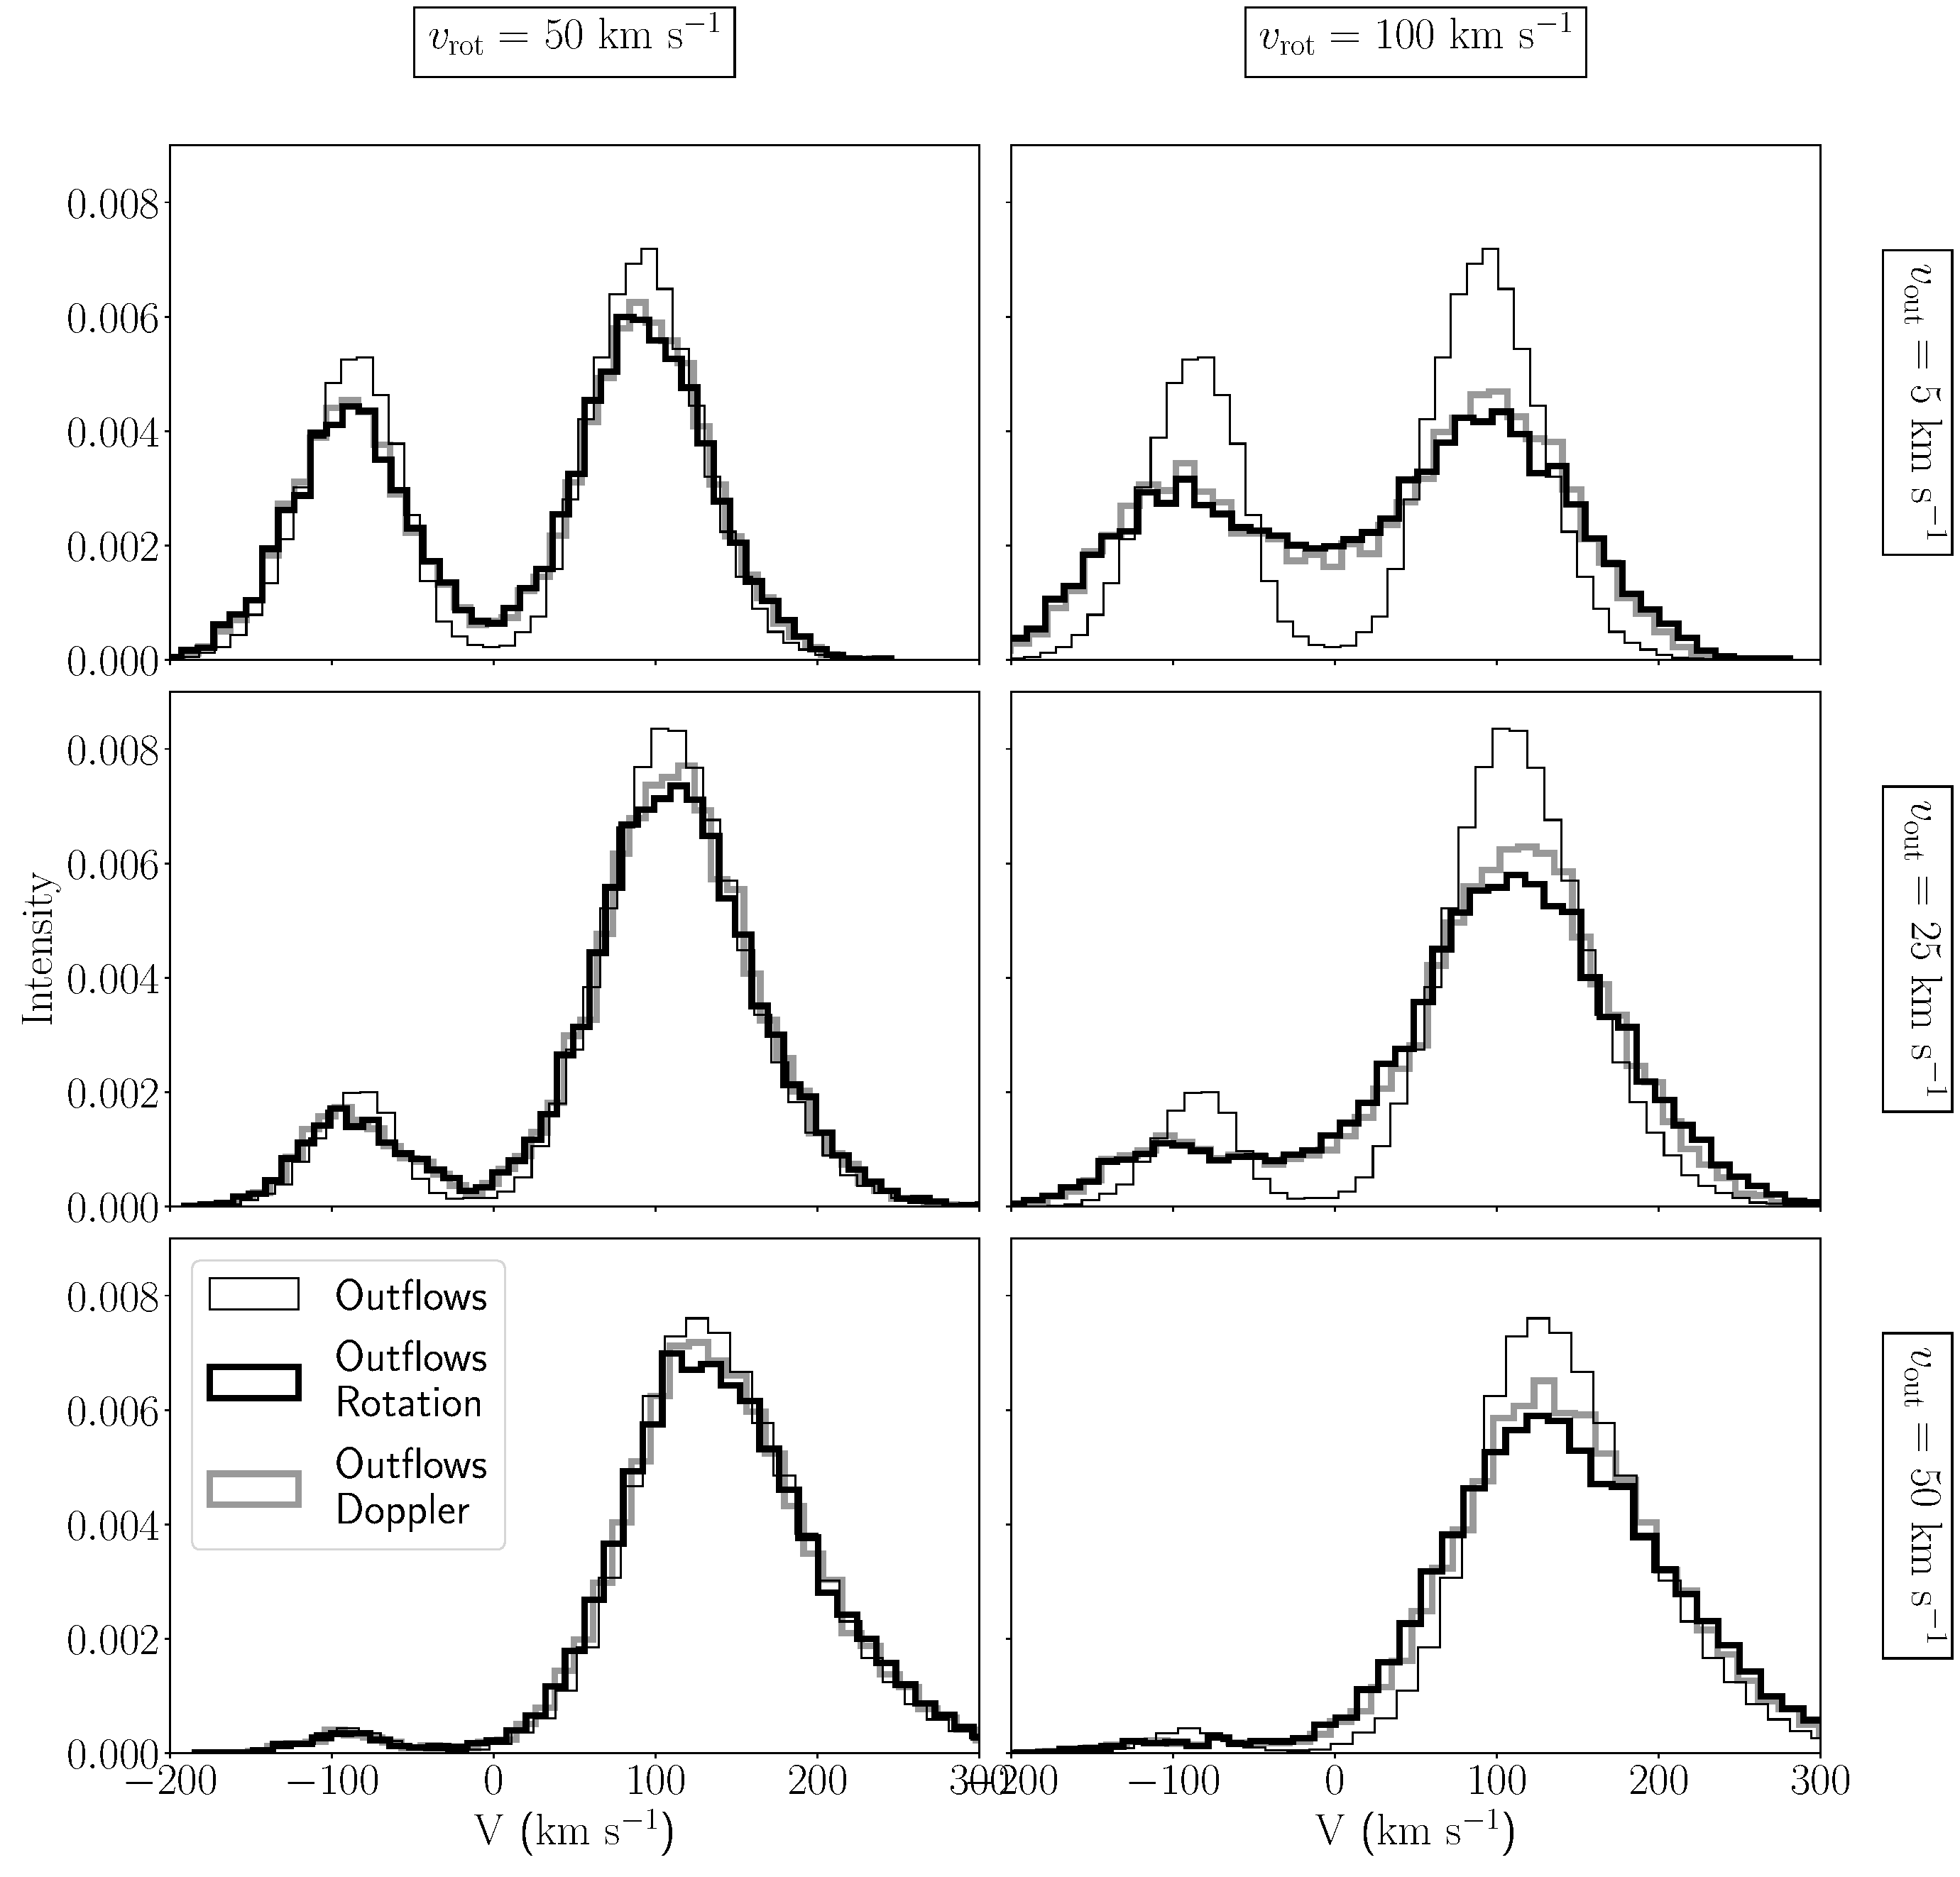
\includegraphics[width=0.90\textwidth]{./figures/results/doppler_shift_logtau6_theta90}
  \end{center}
  \caption{\textbf{Qualitative trends of changing outflow and
      rotational velocity}. 
    Here we fix $\tauh=10^6$ and $\theta=90^\circ$.
    We vary \vrot increasing from left to right and \vout increasing from top to
    bottom. 
    The thin black line corresponds to the \lya line obtained with
    CLARA without any rotation and the indicated outflow velocity.
    The thick black line corresponds to the results including both
    outflows and rotation.
    The thick gray line shows the results of modifyin the pure outflow
    solution by the Doppler shift presented in Equation \ref{eq:shift_x}
    (in thin line), if there is a radiative transfer of rotation and outflows
    (thick and clear line), and if there is a radiative transfer of only outflows,
    but also a Doppler shift from the rotational velocity (thick and dark line).
    \label{fig:doppler_shift}}
\end{figure*}

\subsection{Quantitative trends}
\label{sec:quantitative}


After finding the qualitative influence of the different parameters.


We evaluate the effects of increasing outflows velocity at fixed
values for the optical depth and rotational velocity.
Figure \ref{fig:varying_outflow_small} summarizes its behavior
(for a largest range see Figure \ref{fig:varying_outflow}).
All plots correspond to the same rotation velocity of
$\vrot=50$\kms, rows have constant optical depth and columns
have constant outflows velocity.


Figure \ref{fig:doppler_shift} displays this Doppler shift for six different
configurations with a fixed optical depth \tauh. In each cell of the grid
there is a \lya spectrum for a galaxy with only outflows and two \lya spectra
for the galaxy with outflows and rotation: one obtained from the radiative
transfer simulation and the other obtained from the Doppler shifting of the
non-rotating galaxy.


% Esta figura deberia tener 2 x 2 vinetas. vrot=50.
% cada panel tiene una curva para theta=0, 45, 90.
% | tau=1E5, vout=25, | tau=1E5, vout=75 |
% | tau=1E6, vout=25, | tau=1E6, vout=75 |
%\begin{figure*}
%\begin{center}
%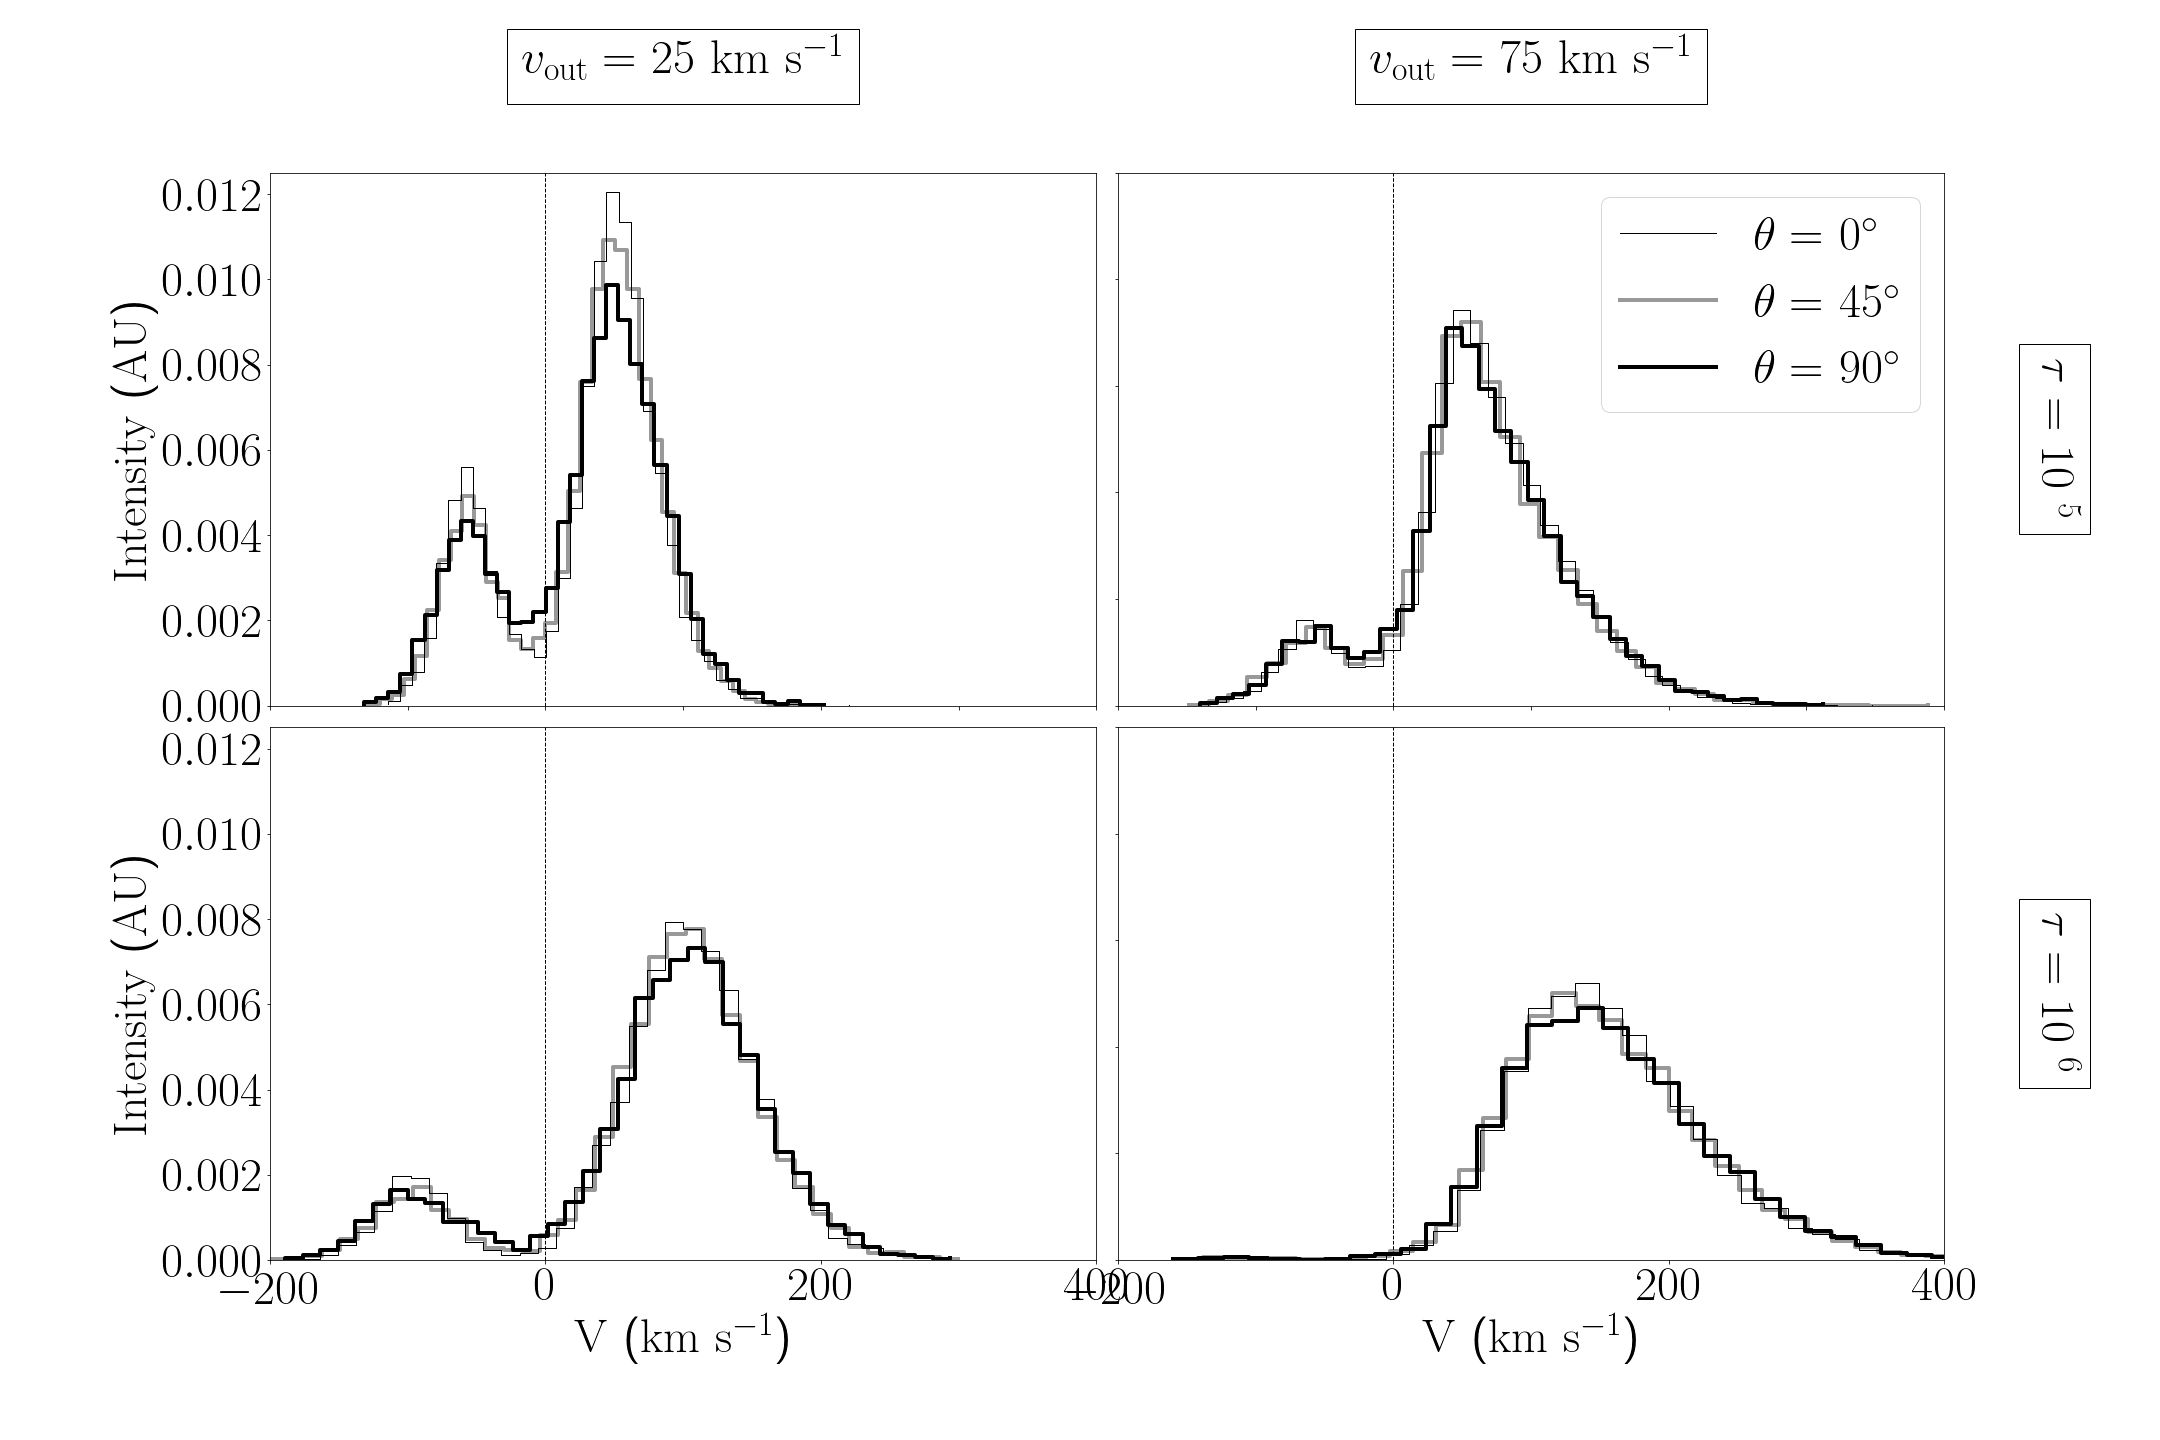
\includegraphics[width=0.90\textwidth]{./figures/results/varying_outflow_small}
%\end{center}
%\caption{\textbf{Spectra for fixed rotational velocity:} We fixed $\vrot=50$\kms.  We vary \vout in%creasing from left to right, \tauh increasing from top to
			 bottom, and $\theta$ according to the legend.
%\label{fig:varying_outflow_small}}
%\end{figure*}


\subsection{Doppler Shifts to Include Rotational Effects}


% Esta figura deberia tener 3 x 2 viñetas. tau=10E6.
% cada panel tiene una curva para no rotation, rotation (radiative transfer)
% y rotation (doppler)
% |vrot=50, vout=5,  | vrot=100, vout=5,  |
% |vrot=50, vout=25, | vrot=100, vout=25, |
% |vrot=50, vout=50, | vrot=100, vout=50, |


In order to compare the line created with the radiative transfer (RT) process that
involves the rotation and the line with only outflows that is Doppler
shifted (DS), we calculate three main characteristics for each spectrum. We
measure the line's mean velocity, standard deviation and skewness for both
RT's and DS's approaches. We plot the results for each value in Figures
\ref{fig:mean_line}, \ref{fig:standard_deviation} and \ref{fig:skewness},
respectively for $\tauh = 10^7$. We highlight that these 3 plots increase
their fit tendency with a higher optical depth. The reasons why will be
discussed in section \ref{sec:discussion}.


\begin{figure*}
\begin{center}
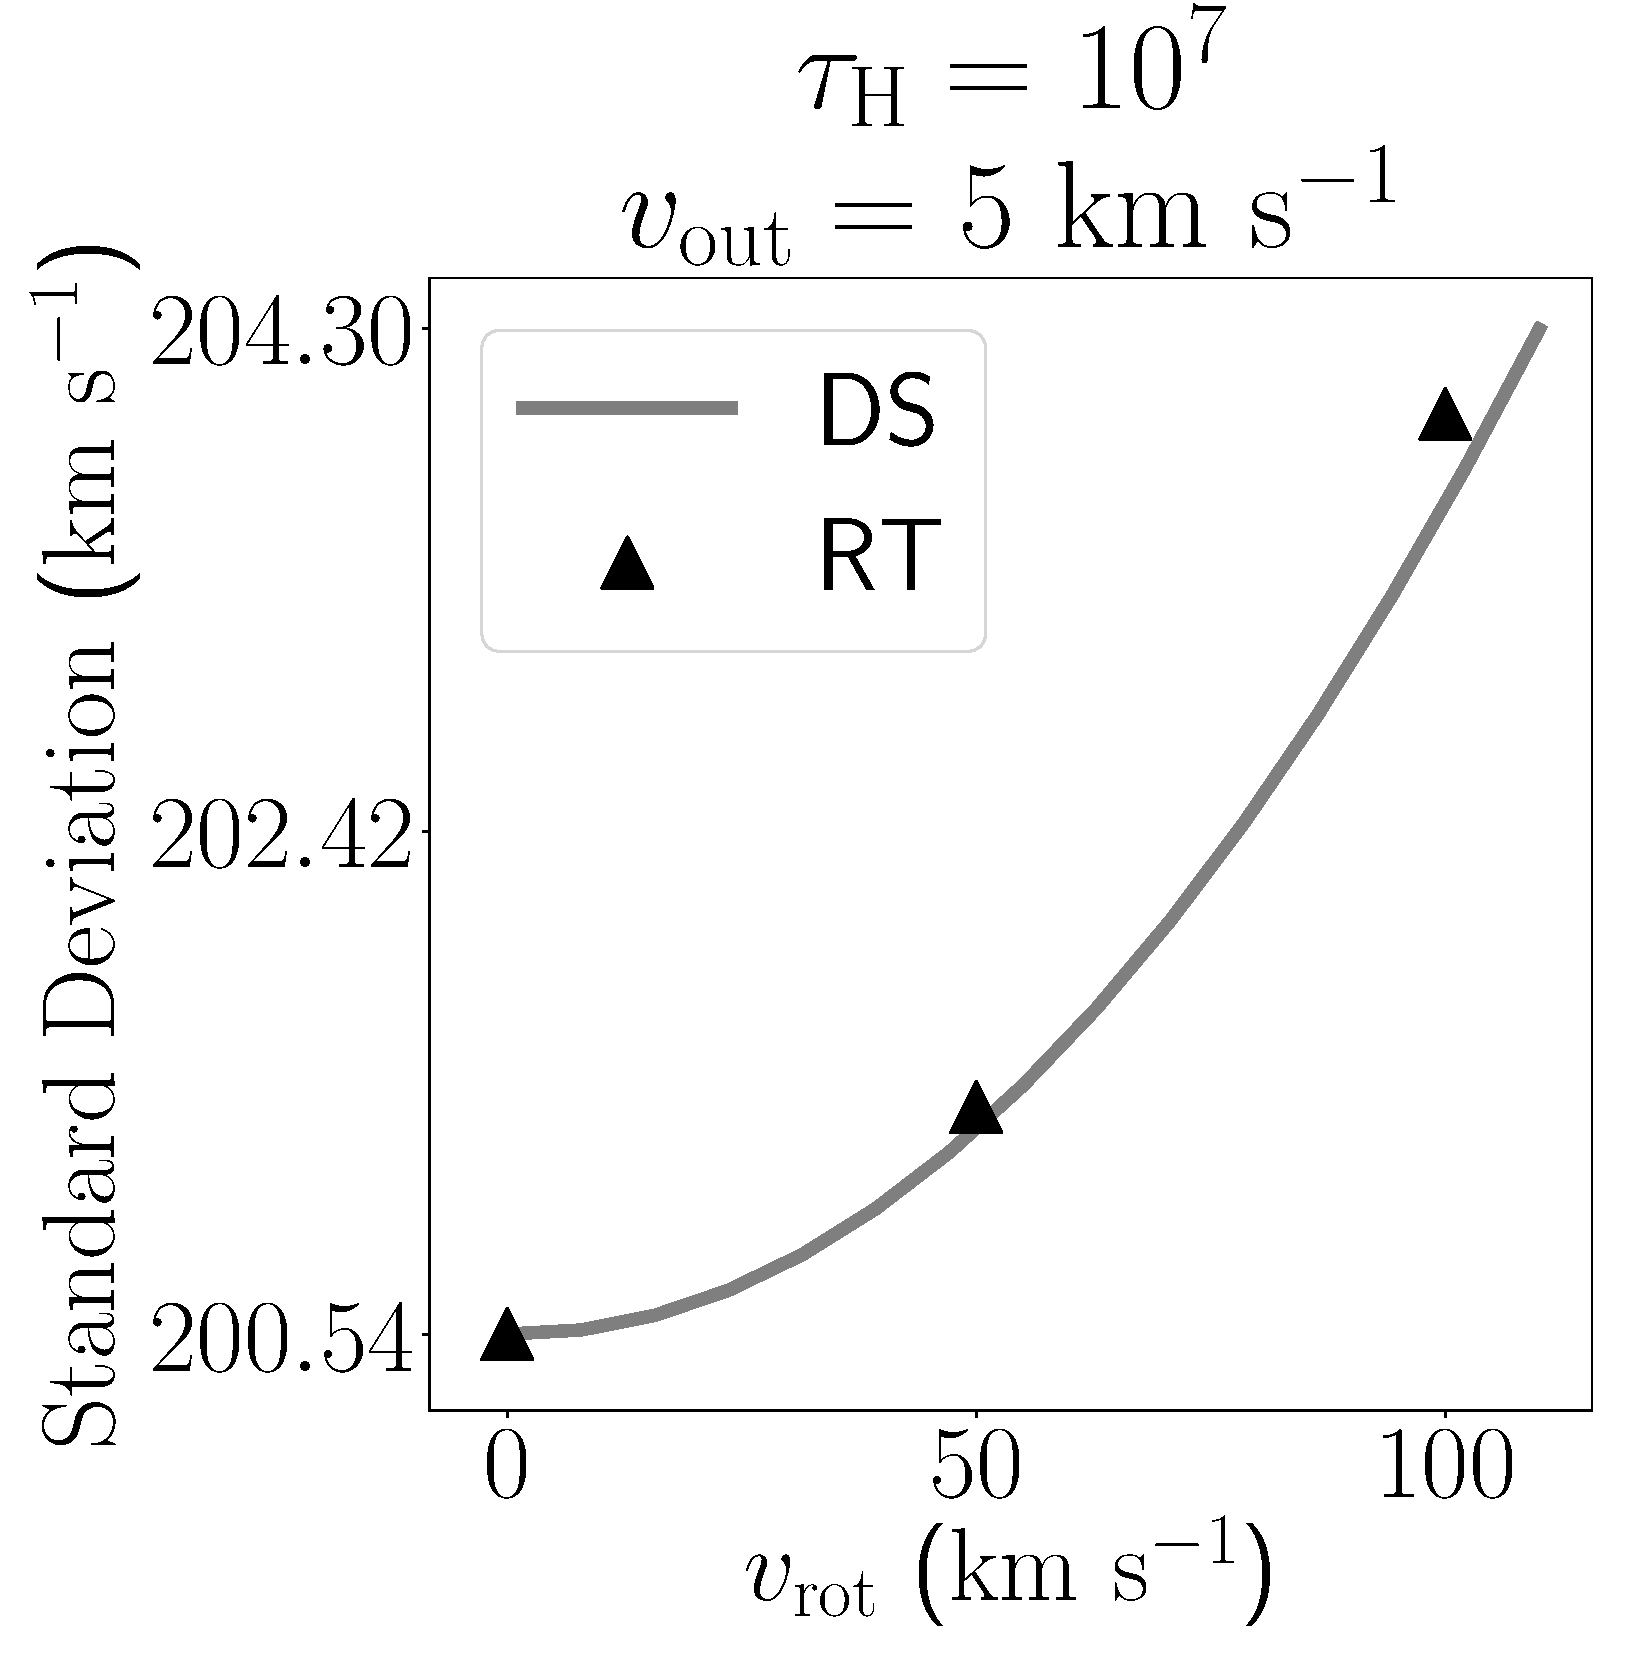
\includegraphics[height=0.3\textwidth]{./figures/results/line_characterization_std_vout5_logtau7}
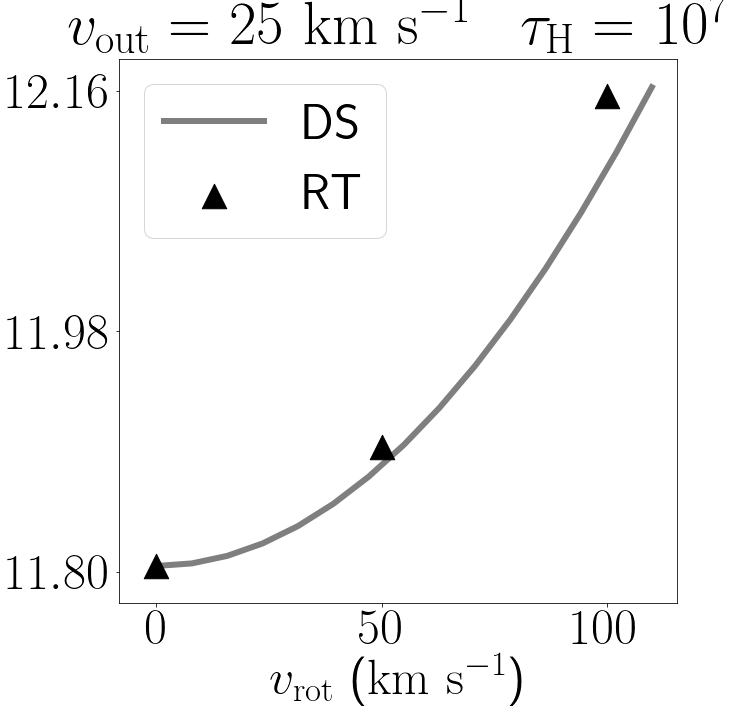
\includegraphics[height=0.3\textwidth]{./figures/results/line_characterization_std_vout25_logtau7}
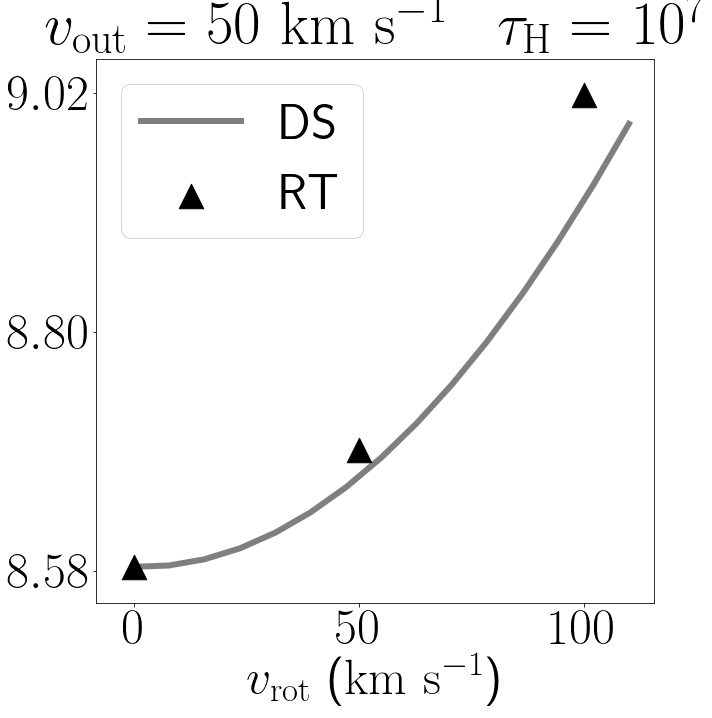
\includegraphics[height=0.3\textwidth]{./figures/results/line_characterization_std_vout50_logtau7}
\end{center}
\caption{\textbf{Standard Deviation for RT and DS:} The triangles represent the Radiative
  Transfer and the lines represent the Doppler Shift. We fixed $\tauh=10^7$.
  \label{fig:standard_deviation}}
\end{figure*}

\begin{figure*}
\begin{center}
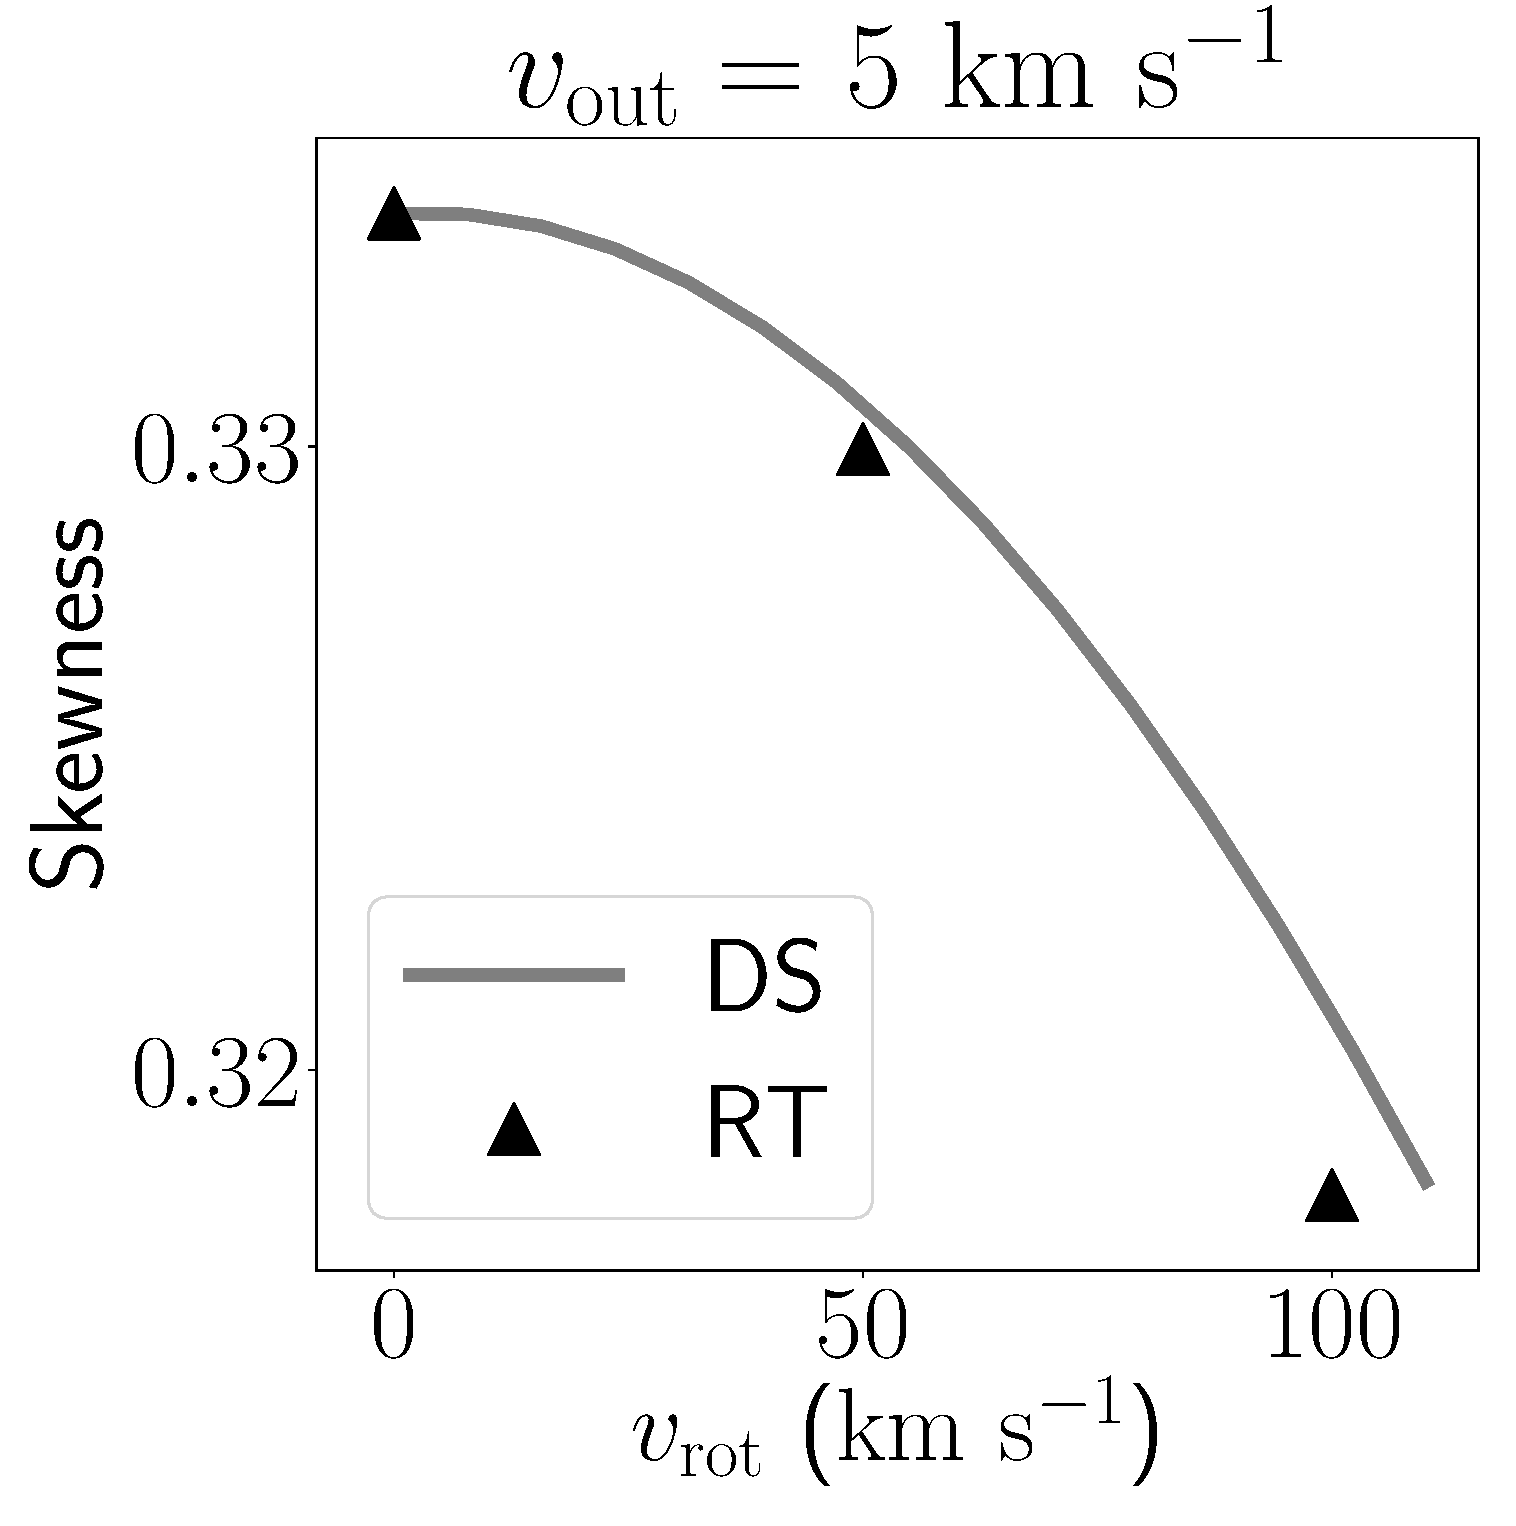
\includegraphics[height=0.31\textwidth]{./figures/results/line_characterization_skw_vout5_logtau7}
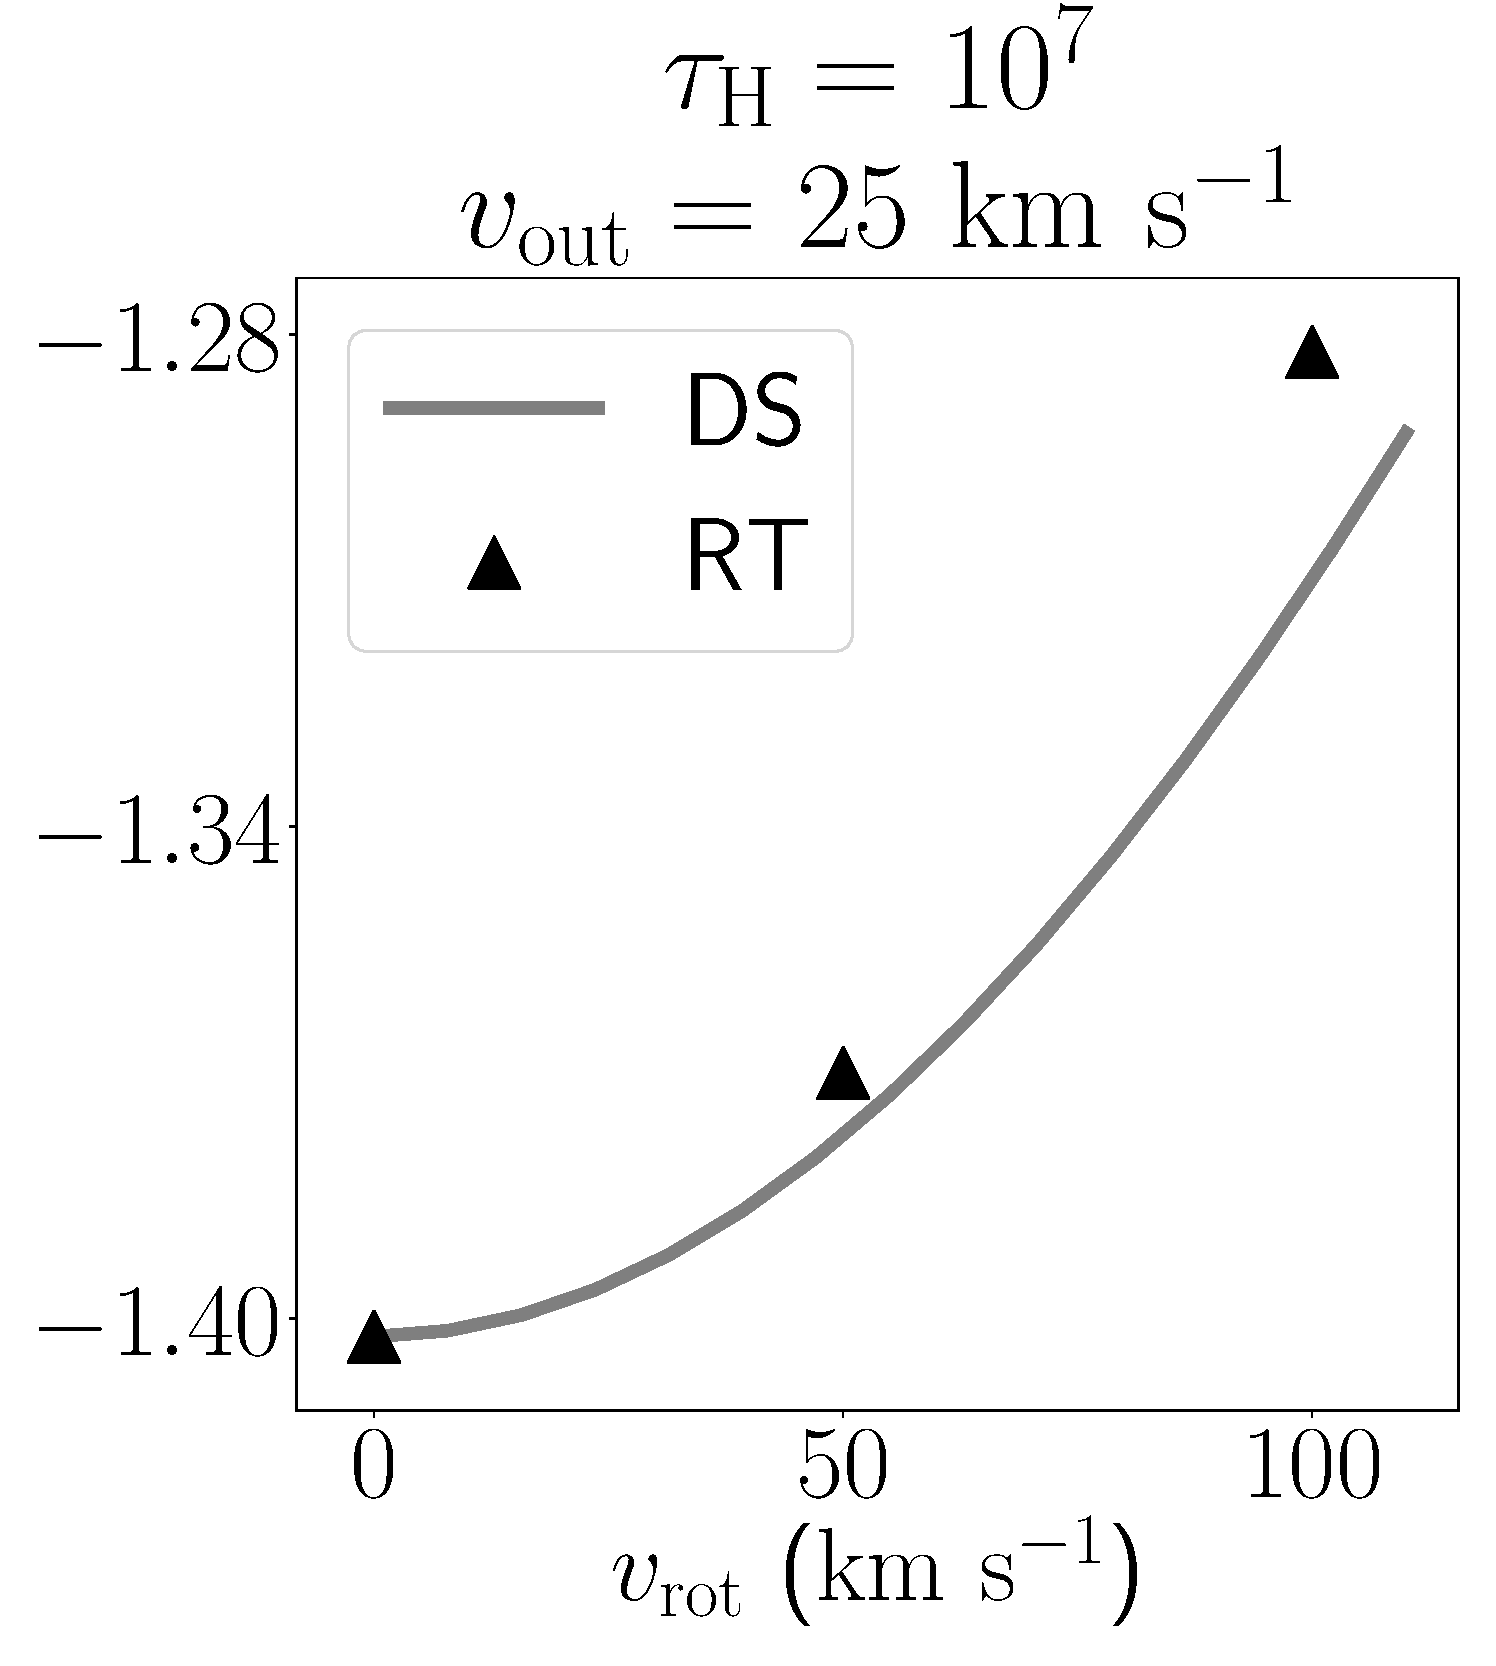
\includegraphics[height=0.31\textwidth]{./figures/results/line_characterization_skw_vout25_logtau7}
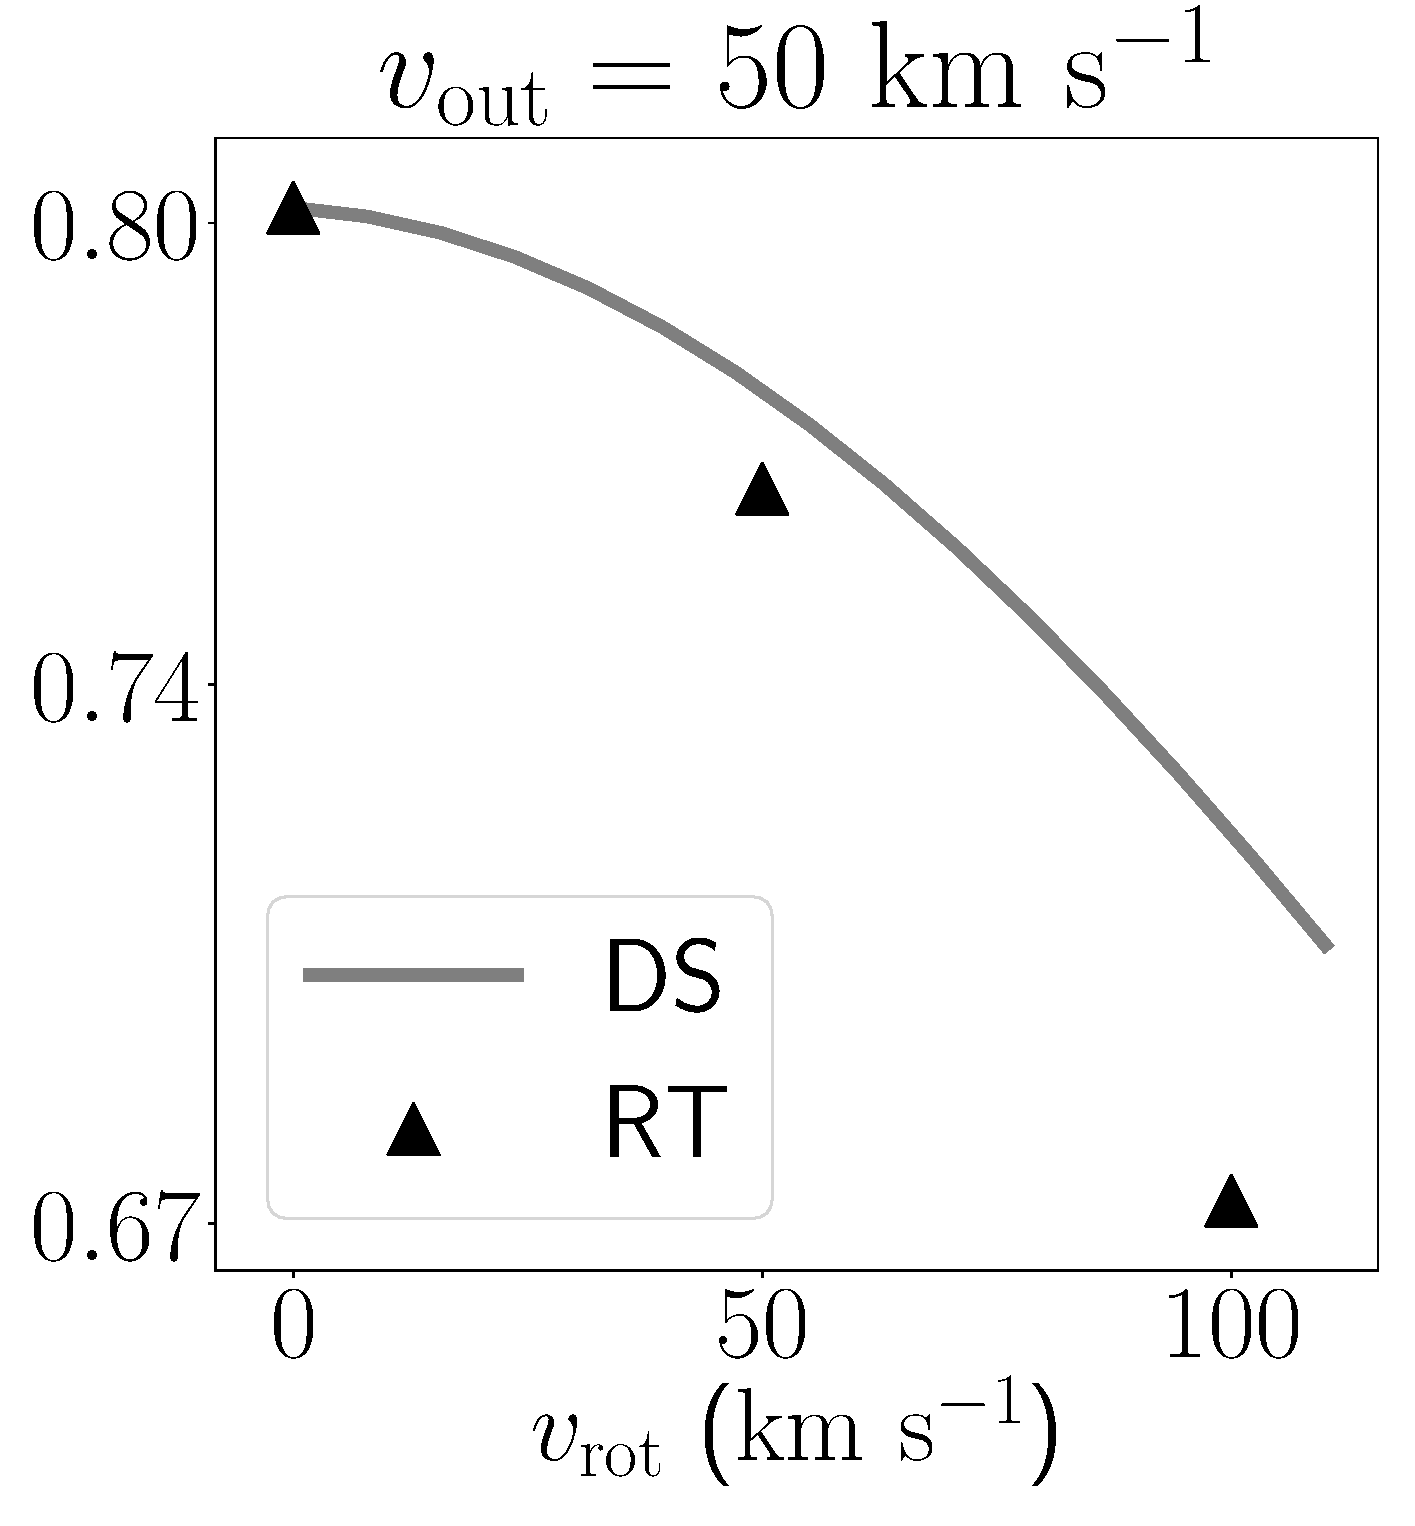
\includegraphics[height=0.31\textwidth]{./figures/results/line_characterization_skw_vout50_logtau7}
  \end{center}
  \caption{\textbf{Skewness for RT and DS:} The triangles represent the Radiative
    Transfer and the lines represent the Doppler Shift. We fixed $\tauh=10^7$.
    \label{fig:skewness}}
\end{figure*}

This shows that the DS model can reproduce the main characteristics of the
RT one. Because of this, we can introduce rotation effects in any spectra
without running the radiative transfer simulations, that usually take a
significant amount of time and computational resources.

In addition to this, we also evaluate the effects of the viewing angle
for fixed rotational and outflows velocity. We measure the intensity of the
valley between peaks, for each $\theta$ and \tauh. Figure \ref{fig:valley_intensity}
summarizes the information with all plots corresponding to the same outflow
velocity of $\vout=5$\kms and rotation velocity of $\vrot=100$\kms.

% Esta figura deberia tener en el eje x theta y en el eje y intensity of valley
% cada panel tiene una curva para logtau = 5, 6, 7.
\begin{figure*}
\begin{center}
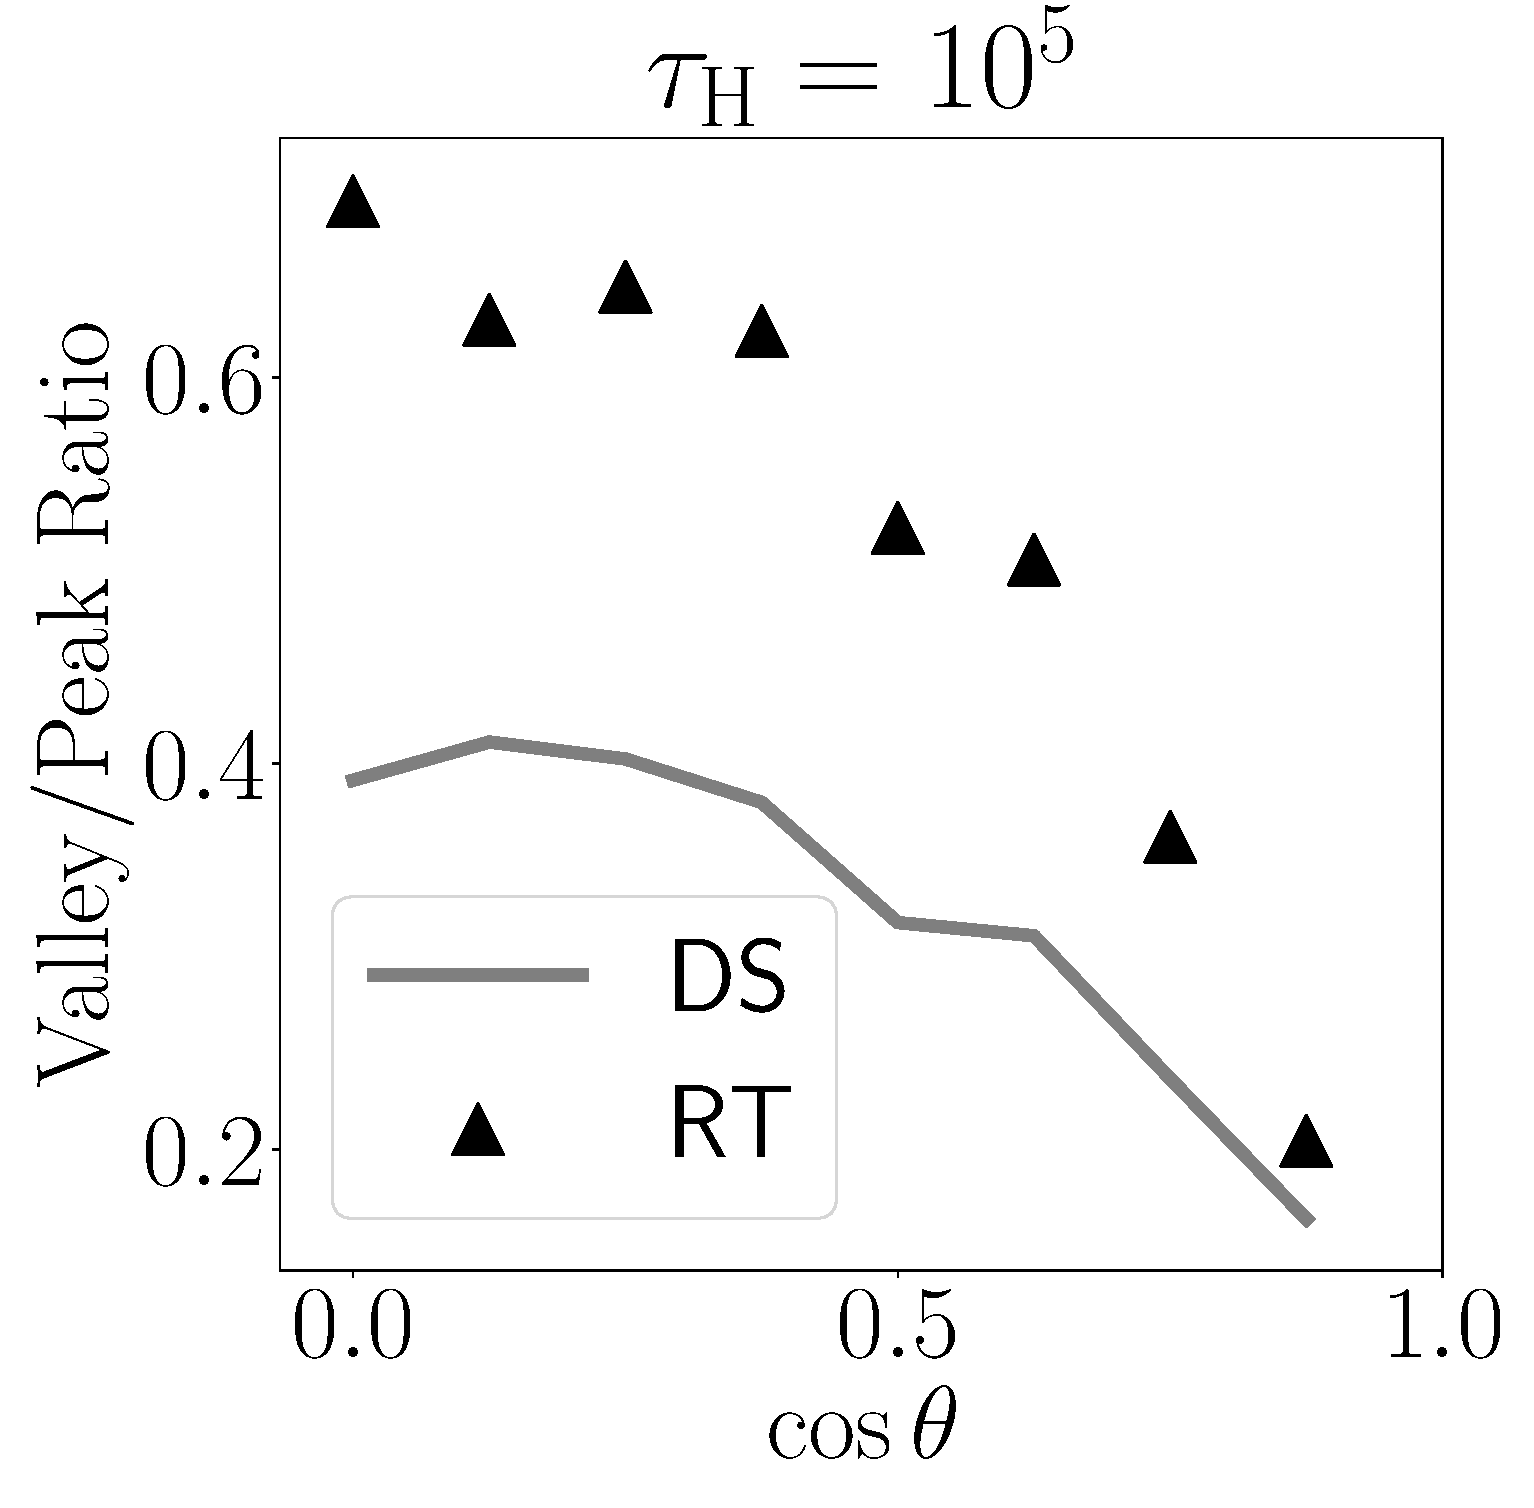
\includegraphics[height=0.29\textwidth]{./figures/results/line_characterization_vi_vout5_vrot100_logtau5}
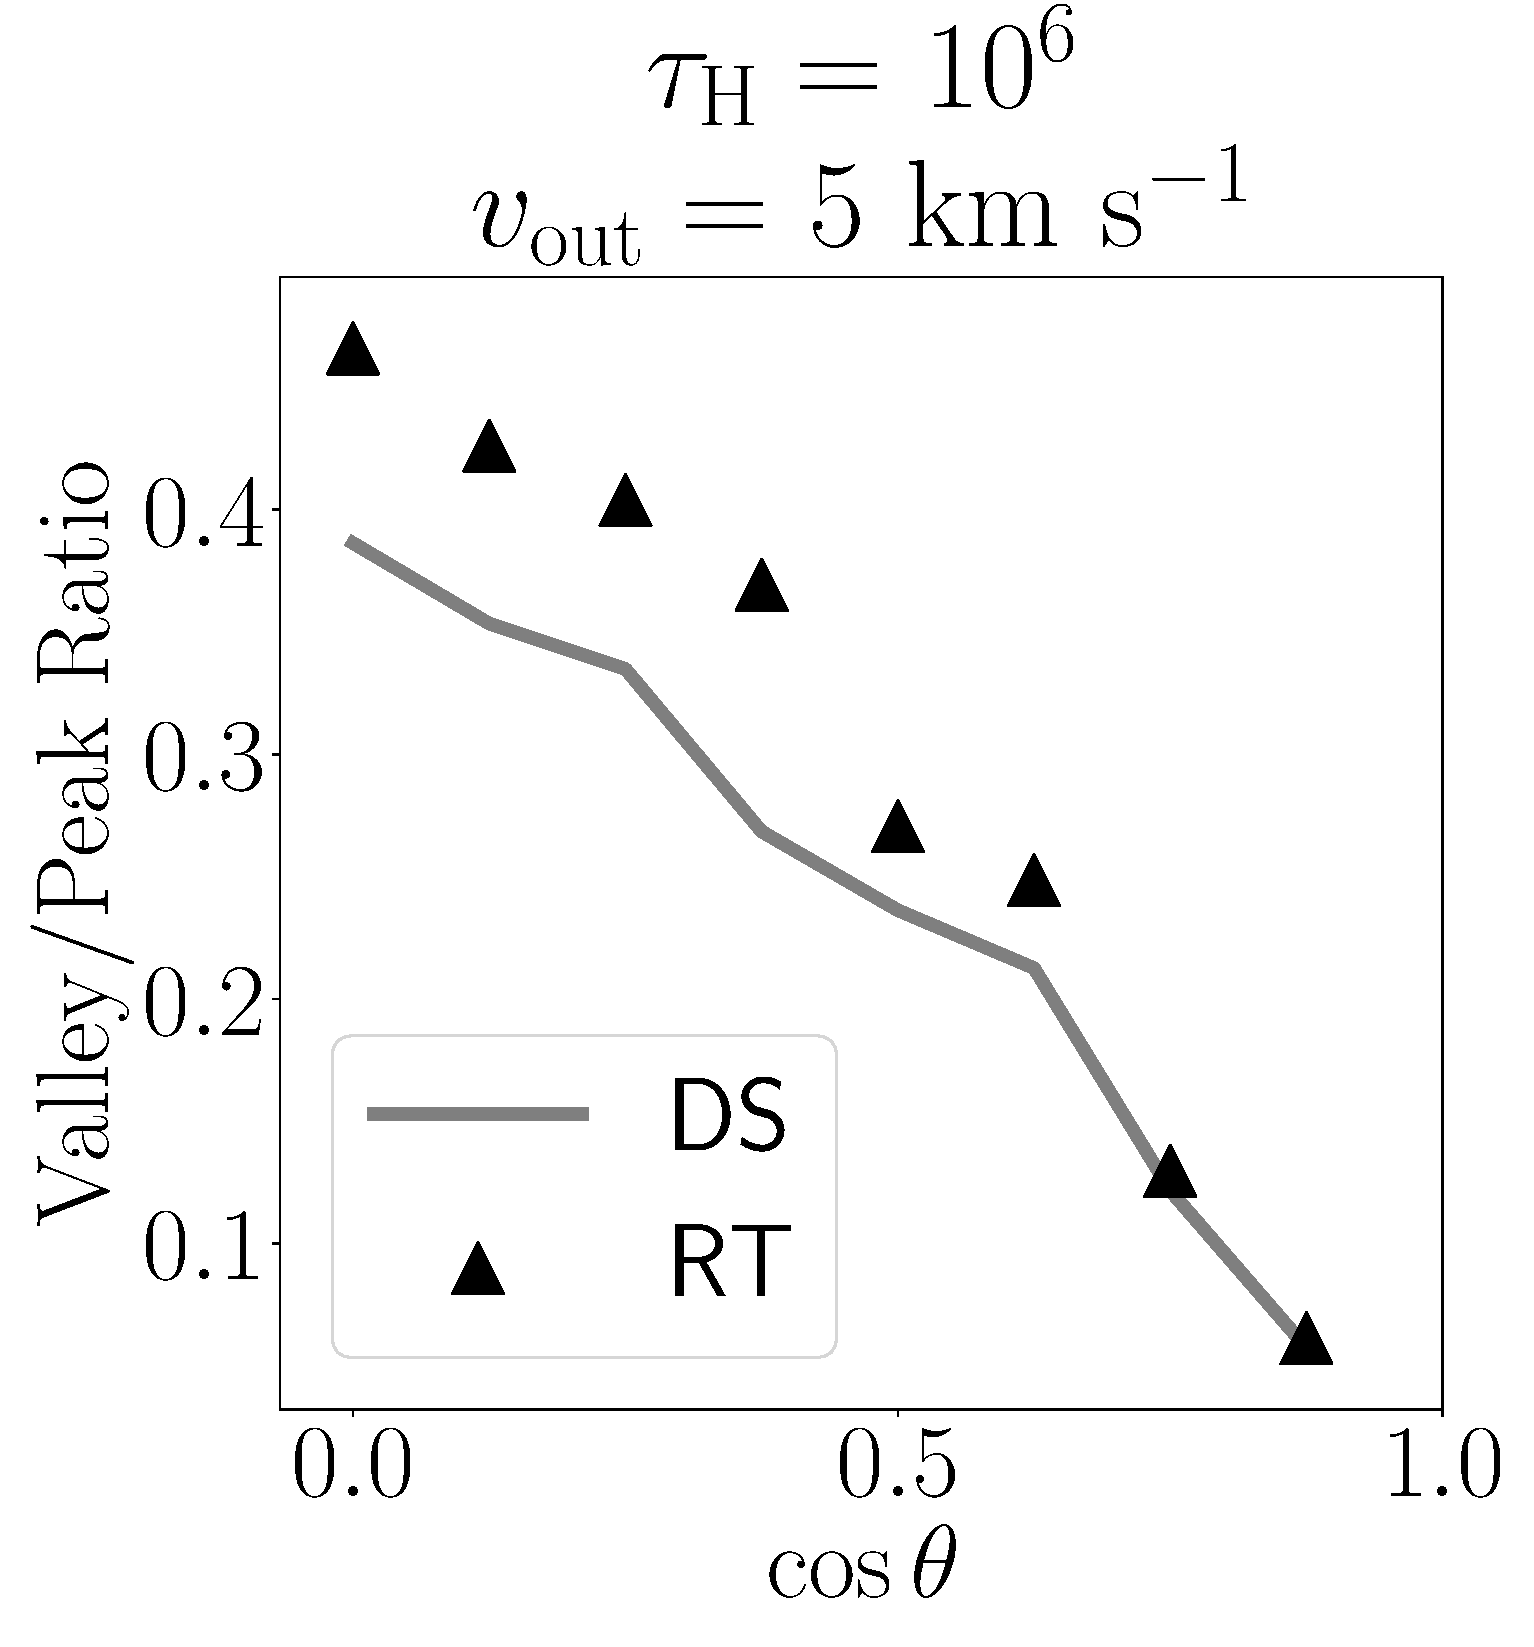
\includegraphics[height=0.29\textwidth]{./figures/results/line_characterization_vi_vout5_vrot100_logtau6}
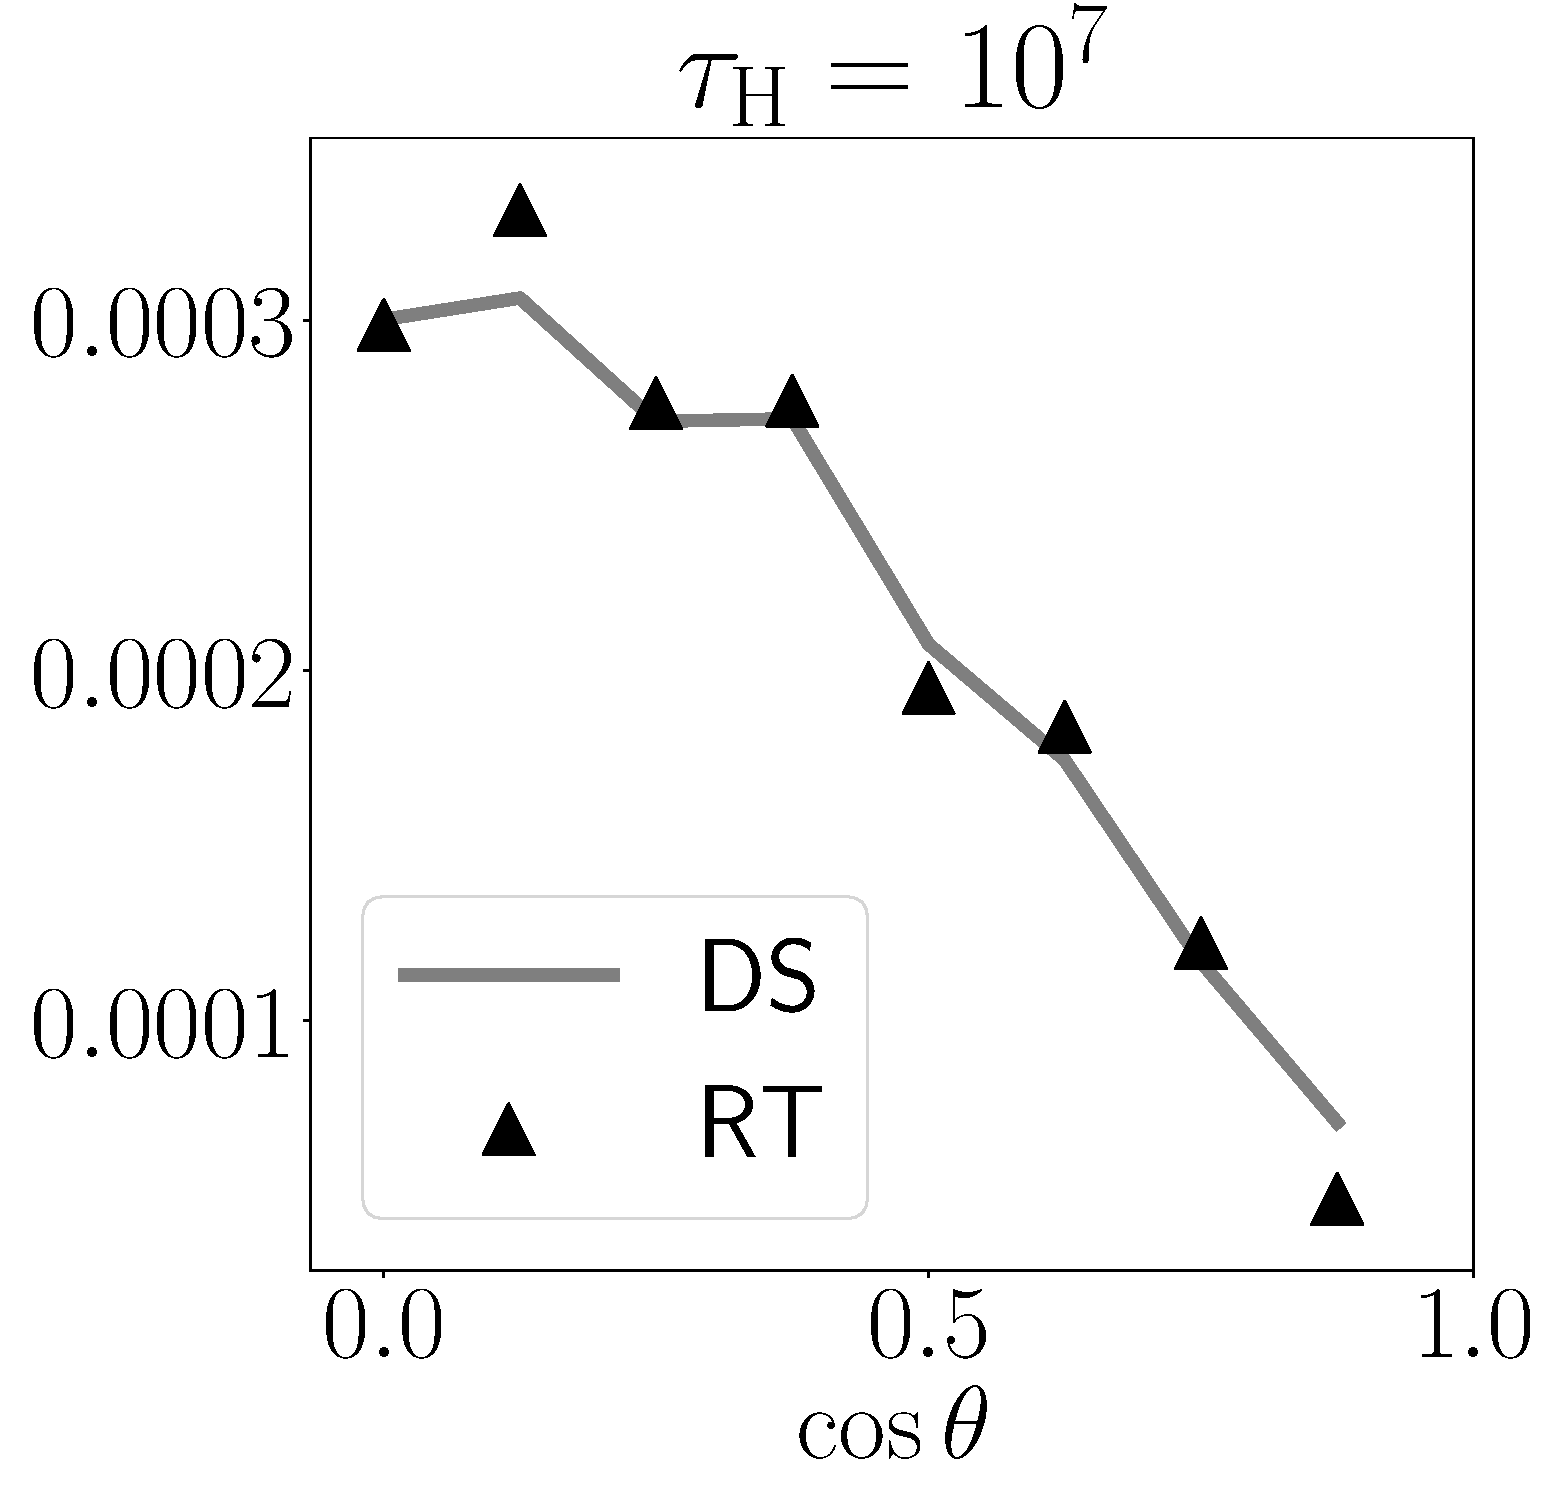
\includegraphics[height=0.29\textwidth]{./figures/results/line_characterization_vi_vout5_vrot100_logtau7}
\end{center}
\caption{\textbf{Valley Intensity:} We show for each \tauh the dependency that
		the viewing angle $\theta$ has on the line's the valley intensity. The larger
		$\cos{\theta}$ the lower is the valley intensity, so the higher $\theta$, the
		higher the valley intensity. We fixed $\vout=5$\kms and $\vrot=100$\kms.
		\label{fig:valley_intensity}}
\end{figure*}


\section{Discussion}
\label{sec:discussion}

\subsection{Theoretical Insights}
\color{red}
Why Doppler Shift works. Talk about radiative transfer...
\color{black}
In Fig. \ref{fig:doppler} we present the spectrum of a LAE taken from to different
sides of the galaxy. As the LAE is rotating, one side is being redshifted while
the other is blueshifted. We see that the combined spectrum is a weighted line,
in solid black, that combines these past two. This shows that there is in fact a
Doppler Shift and then it justifies our choice to apply it after the outflows spectrum is
obtained.

\begin{figure}
	\begin{center}
		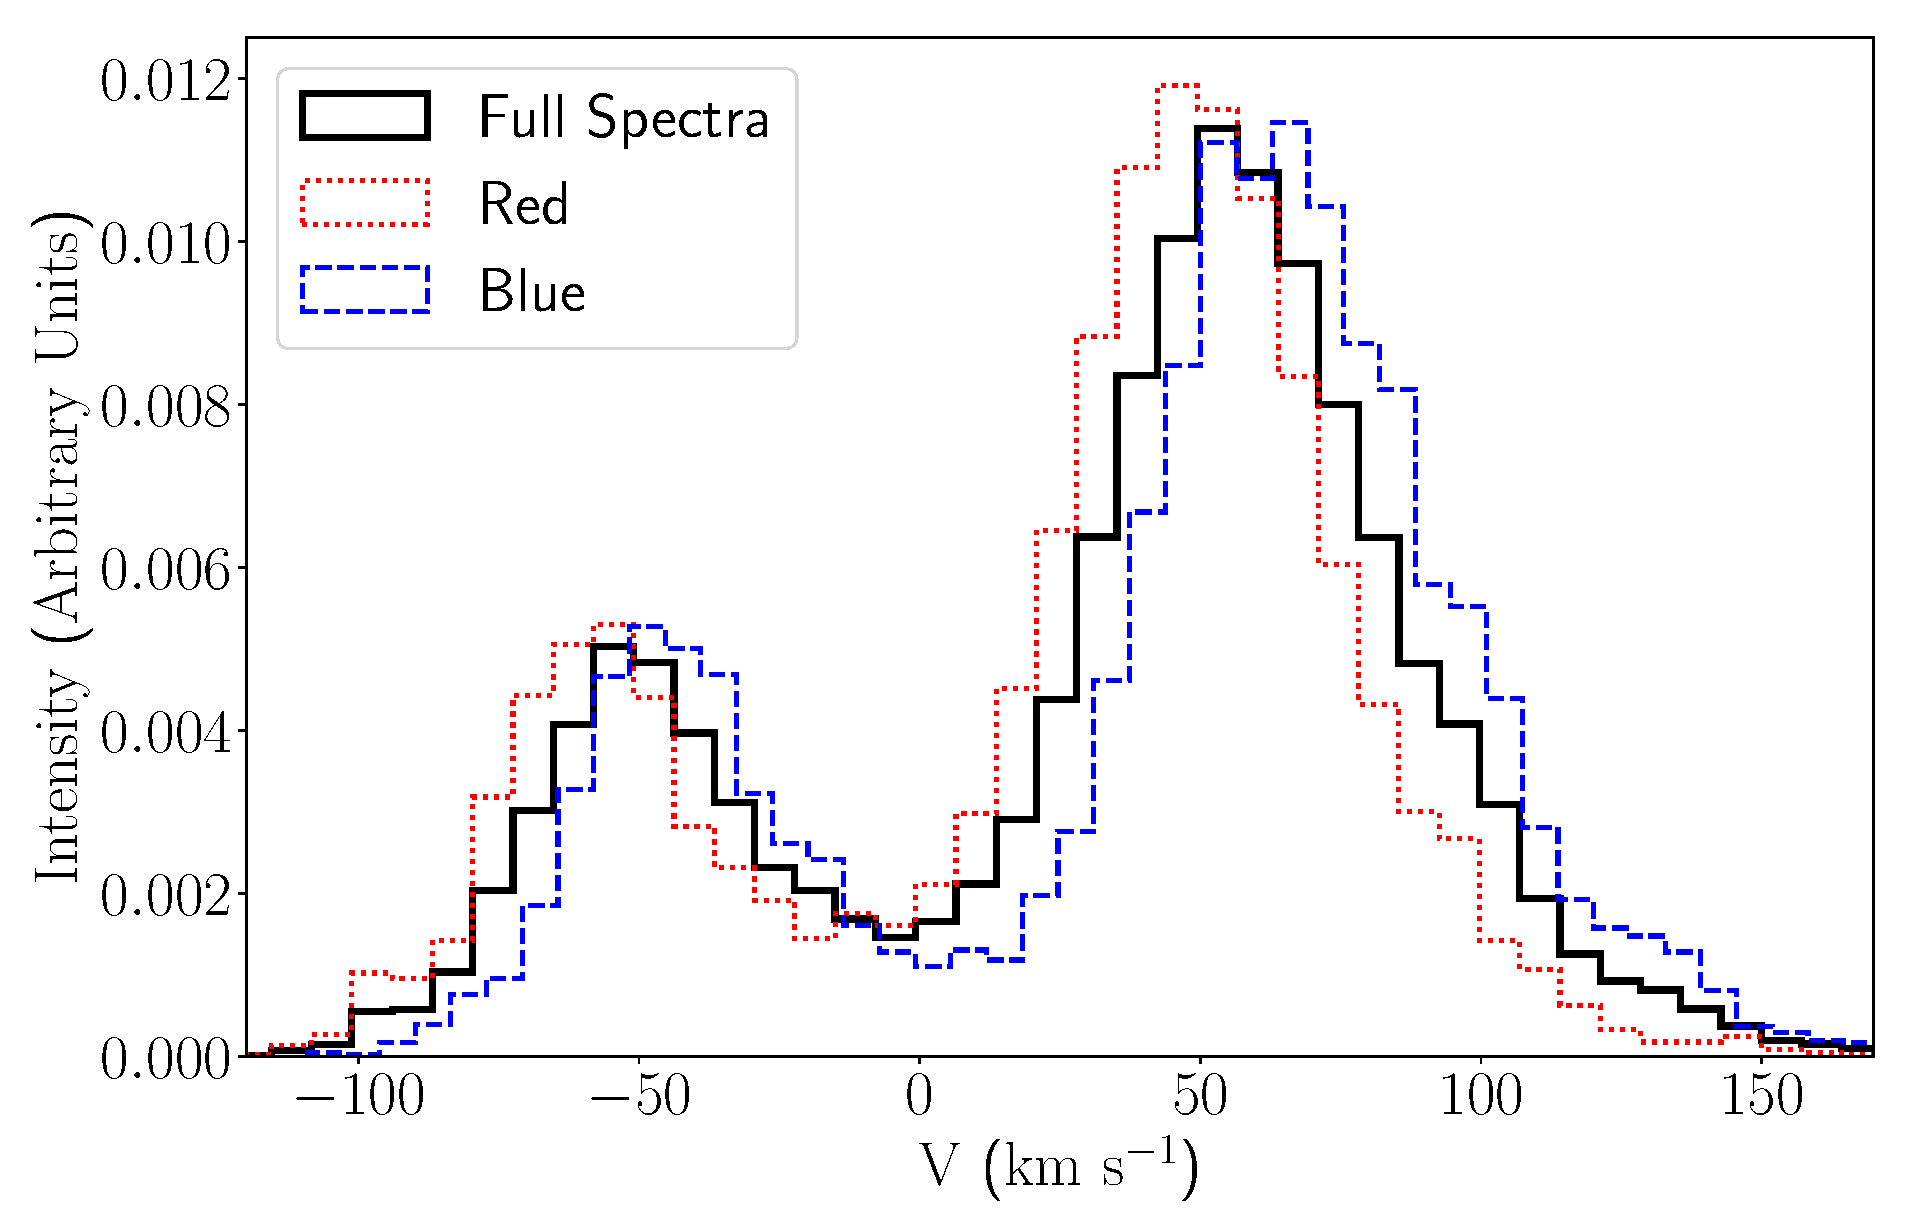
\includegraphics[width=0.48\textwidth]{./figures/discussion/doppler}
	\end{center}
	\caption{\textbf{Doppler Shift:} We fix $\vout=25$\kms, $\vrot=100$\kms, $\tauh=10^5$.
		\label{fig:doppler}}
\end{figure}

A first approach to an analytical expression that returns the \lya spectrum
from a rotating galaxy is presented by \cite{Garavito14}. This derivation is
based on the assumption that the distribution of photons' propagation directions
at the edge of the galaxy is anisotropic and depends of \tauh only. So this
approximation becomes more accurate with higher optical depth and it is also the
reason why the Doppler Shift technique to induce rotational effects to an outflow
\lya spectrum works.

On the other hand, regarding the parameters \vrot, \vout, and $\theta$ for
which this model would work, we have the following. The effect of the outflows
velocity is much more sensitive on the spectrum than the rotational one; meaning
that for a high \vout, the \vrot value would have to be equal or greater in order
to be able to glimpse the shift in frequency that rotation induces. Regarding $\theta$,
the introduction of rotation in the model implies that it will only affect galaxies
with its viewing angle $\theta \neq 90^\circ$. This can be observed in the cartesian
components of the velocity of the atoms (Eq. \ref{eq:vx}, \ref{eq:vy}, \ref{eq:vz})
where the only velocity factor affecting $v_z$ is the outflows one.

\subsection{Application to observational data}

We find three different approaches how this model can have observational
implications. Firstly, as the resolution of astronomical instruments is
increasing, new images from LAEs can be spatially resolved in a way that
rotation velocities of the galaxy can be determined. New spectrographs like
MUSE should help obtain kinematic information from LAEs by using our model.
As for now, previous works in the literatures have already found useful data
to support this idea. Fig 7 of Prescott et al. \cite{Prescott14} shows the
presence of Doppler shift and \cite{Herenz2016} creates 2D line of sight
velocity maps of several LARS (Lyman Alpha Reference Sample) galaxies.

Another application of this new model to the current interpretation of \lya
spectra, is that the central ($V=0$) emission of the spectra seen in the
\lya line, is a consequence of the viewing angle of the galaxy and can be
controlled by it. Several authors have suggested that this central emission
is caused by radiation that escapes the galaxy without scattering. So we
present an alternative that solves this issue. In addition, the effect of
outflows velocities \vrot in current models can modify the asymmetry of peaks
present in the \lya line. However the intensity of the valley and the width
of the line were not easily reproduced. In this work we provide a tool to
provide these effects with values of \vout and \vrot that do not exceed the
typical LAEs' values found in the literature.

\color{red}
Kulas...
\color{black}
Finally, we present a reconstruction of a selected \lya spectrum presented
by \cite{Kulas12} and reproduced with the permission of the author. We create
a fit of the \lya line and predict its kinematic properties.

\section{Conclusions}
\label{sec:conclusions}

In this paper we explore, for the first time in the literature,
the results of a model for the emergent \lya\ line from rotating outflows.
The main results for the model are computed from a Monte-Carlo radiative transfer
simulation and confronted with a simple semi-analytic ansatz that adds the effects
of rotation onto results of pure outflow kinematics.

The main effects of rotation on the \lya\ line morphology are:


\begin{itemize}
  \item Broadening the line.
	\item Increasing the intensity at the line's center.
	\item Inducing a dependency on the viewing angle,
  The closer the observer is to the pole of the galaxy (defined by the rotation axis),
  the smaller are the effects from rotation.
\end{itemize}

We found that in the case of solid body rotation these effects can be quantitatively
explained by a Doppler boost, where the Doppler factor can be computed as the
 producet of quantities at the surface of last scattering, namely $\vec{v}_{\rm rot}\cdot \hat{k}$,
 where $\vec{v}_{\rm rot}$ is the velocity due to rotation and $\hat{k}$ is the direction
of the photon's propagation.
These conclusions, specially the confirmation of the Doppler boost as
a good proxy for solid body rotation, strenghten the evidence reported
by \cite{Garavito14} when they modeled the effect of pure rotation on
\lya\ spectra.  

As an application to observational data we find that recent results
that take the spectra of two different sides of a galaxy can detect 
the effect of approaching/receeding gas motions. 
However, the distances between the peaks of these two spectra 
correspond to $\approx v_{\rm rot} \cos\theta$ due to the weights of the
emitting regions.




\bibliographystyle{mnras}
\bibliography{references}


\appendix

\section{Additional figures}
\label{sec:appendix}

In this appendix we show \lya spectra with fixed \vout (Fig. \ref{fig:varying_rotation_small})
and fixed \vrot (Fig. \ref{fig:varying_outflow_small}). For a larger set of spectra with the
same fixed \vout and \vrot refer to Fig. \ref{fig:varying_rotation} and Fig. \ref{fig:varying_outflow}
respectively.

\begin{figure*}
	\begin{center}
		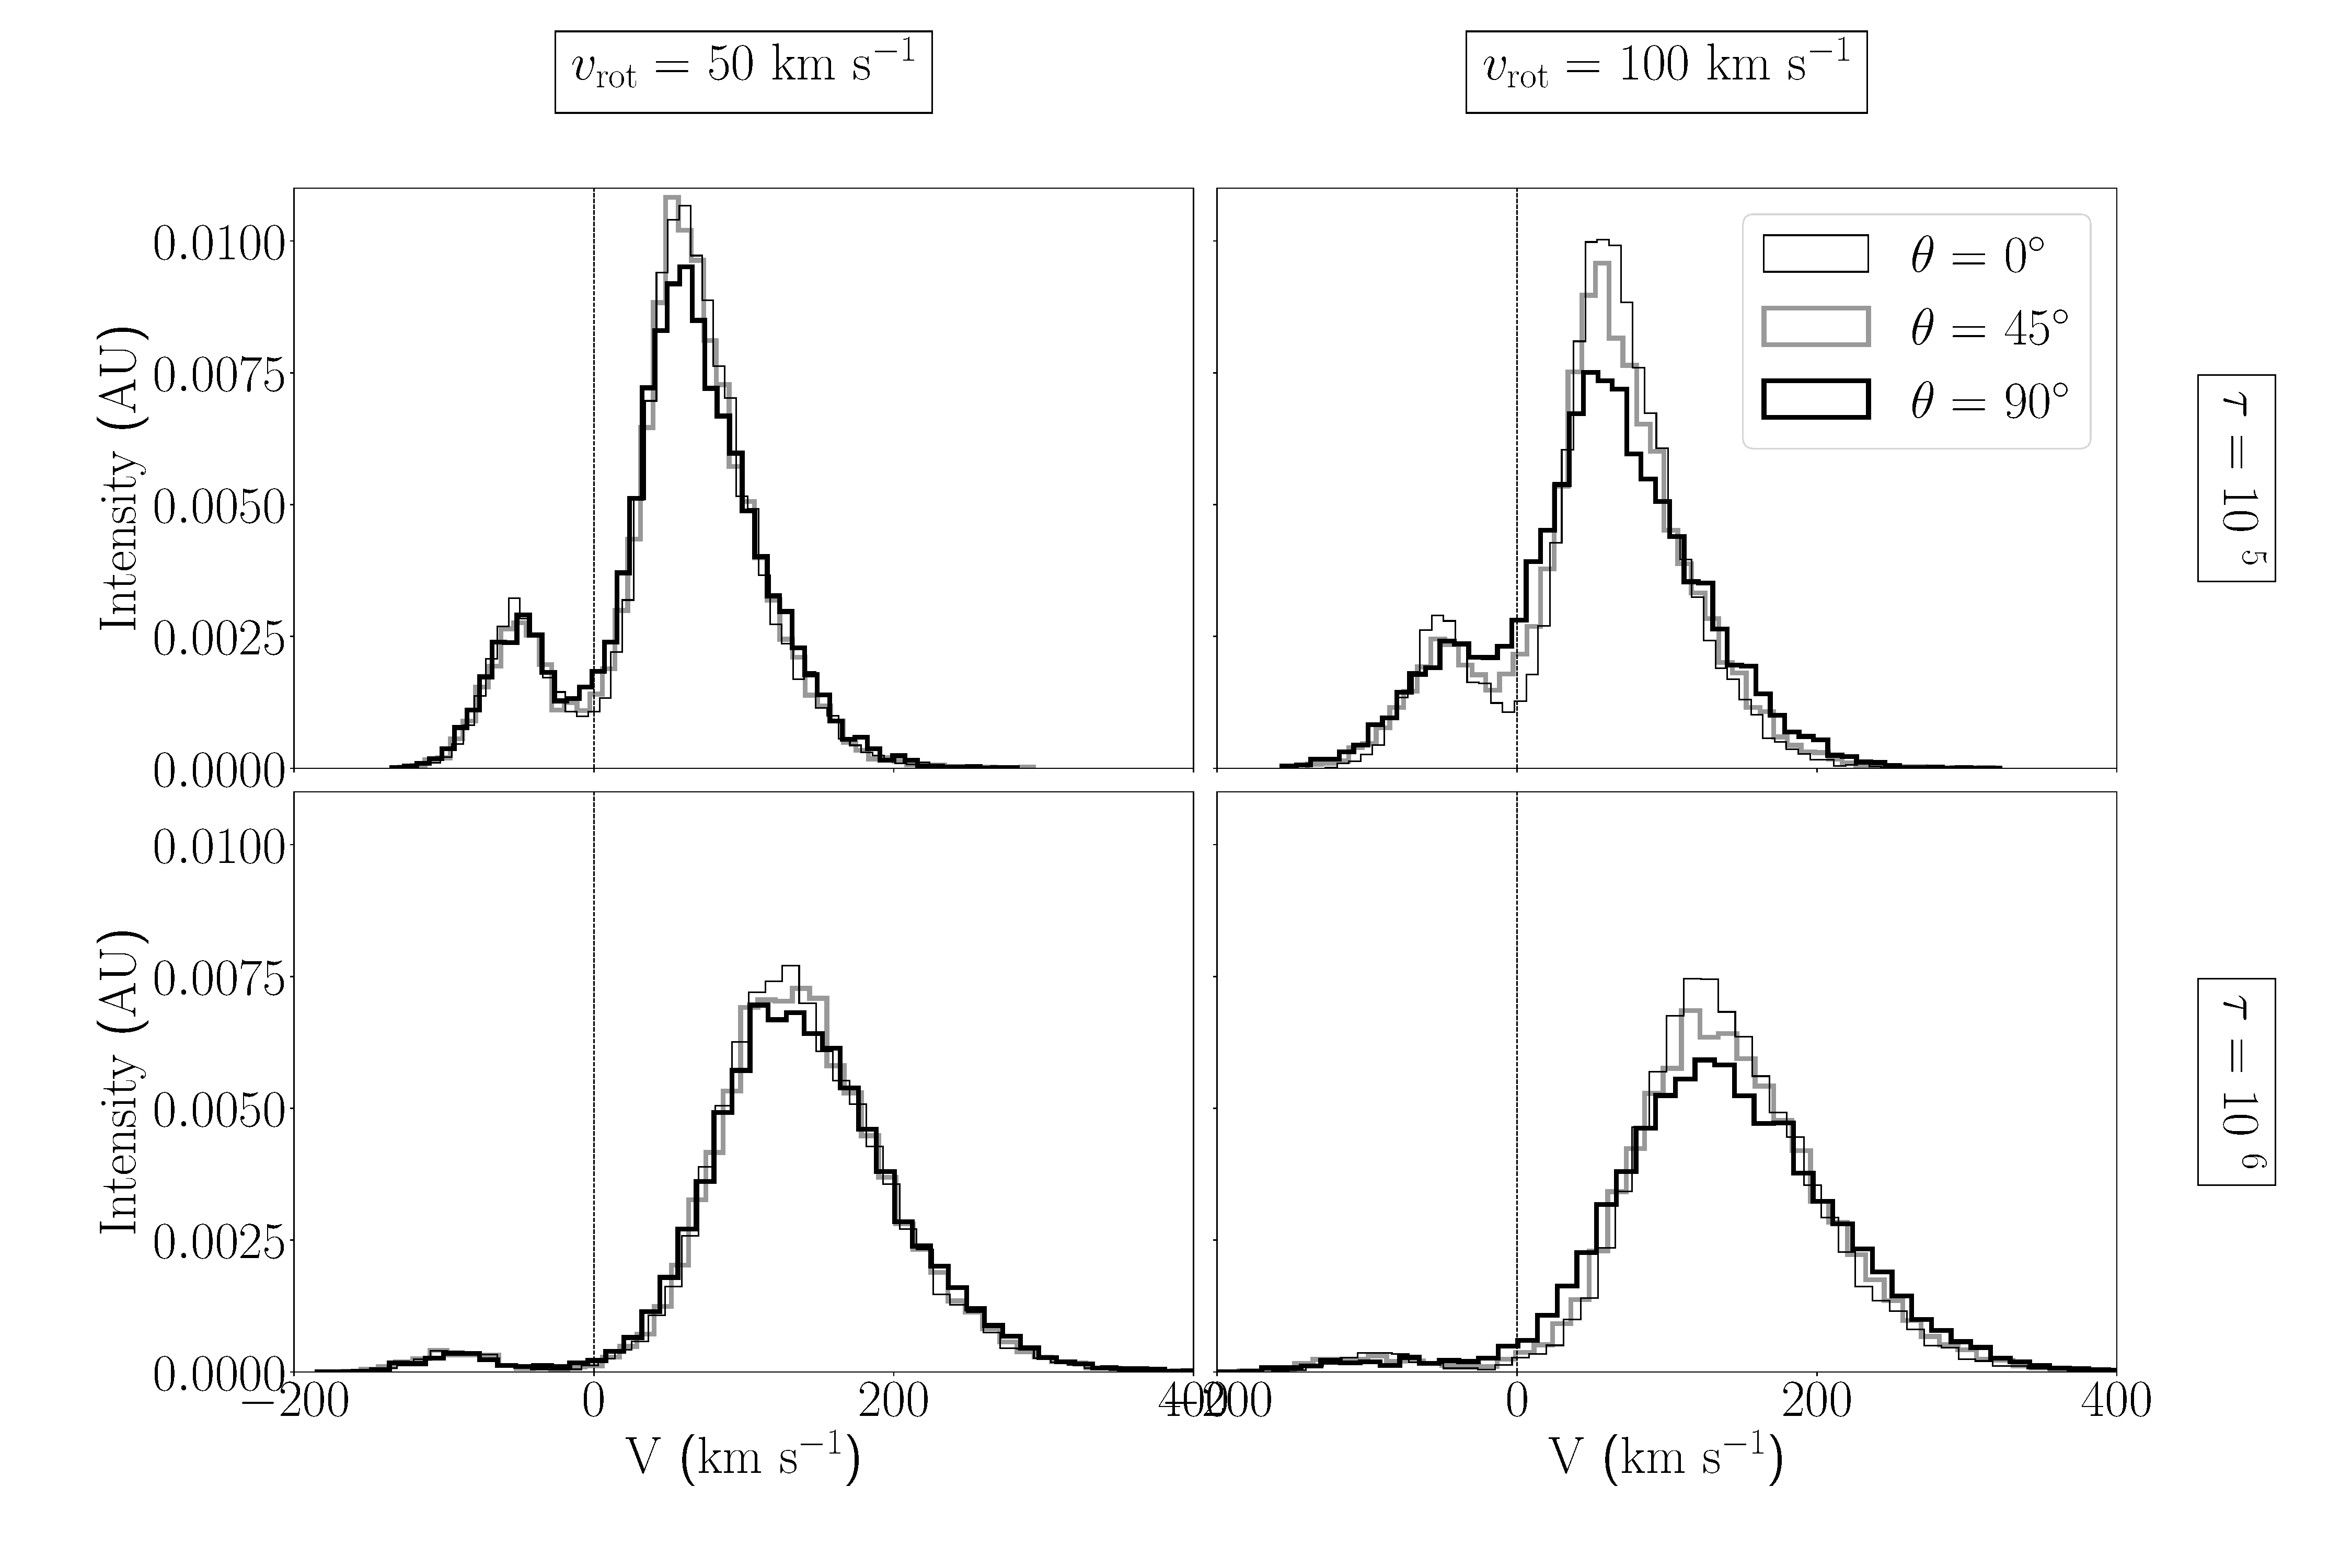
\includegraphics[width=0.90\textwidth]{./figures/appendix/varying_rotation_small}
	\end{center}
	\caption{\textbf{Spectra with fixed outflows velocity:} We fix $\vout=50$\kms.
		\label{fig:varying_rotation_small}}
\end{figure*}

\begin{figure*}
	\begin{center}
		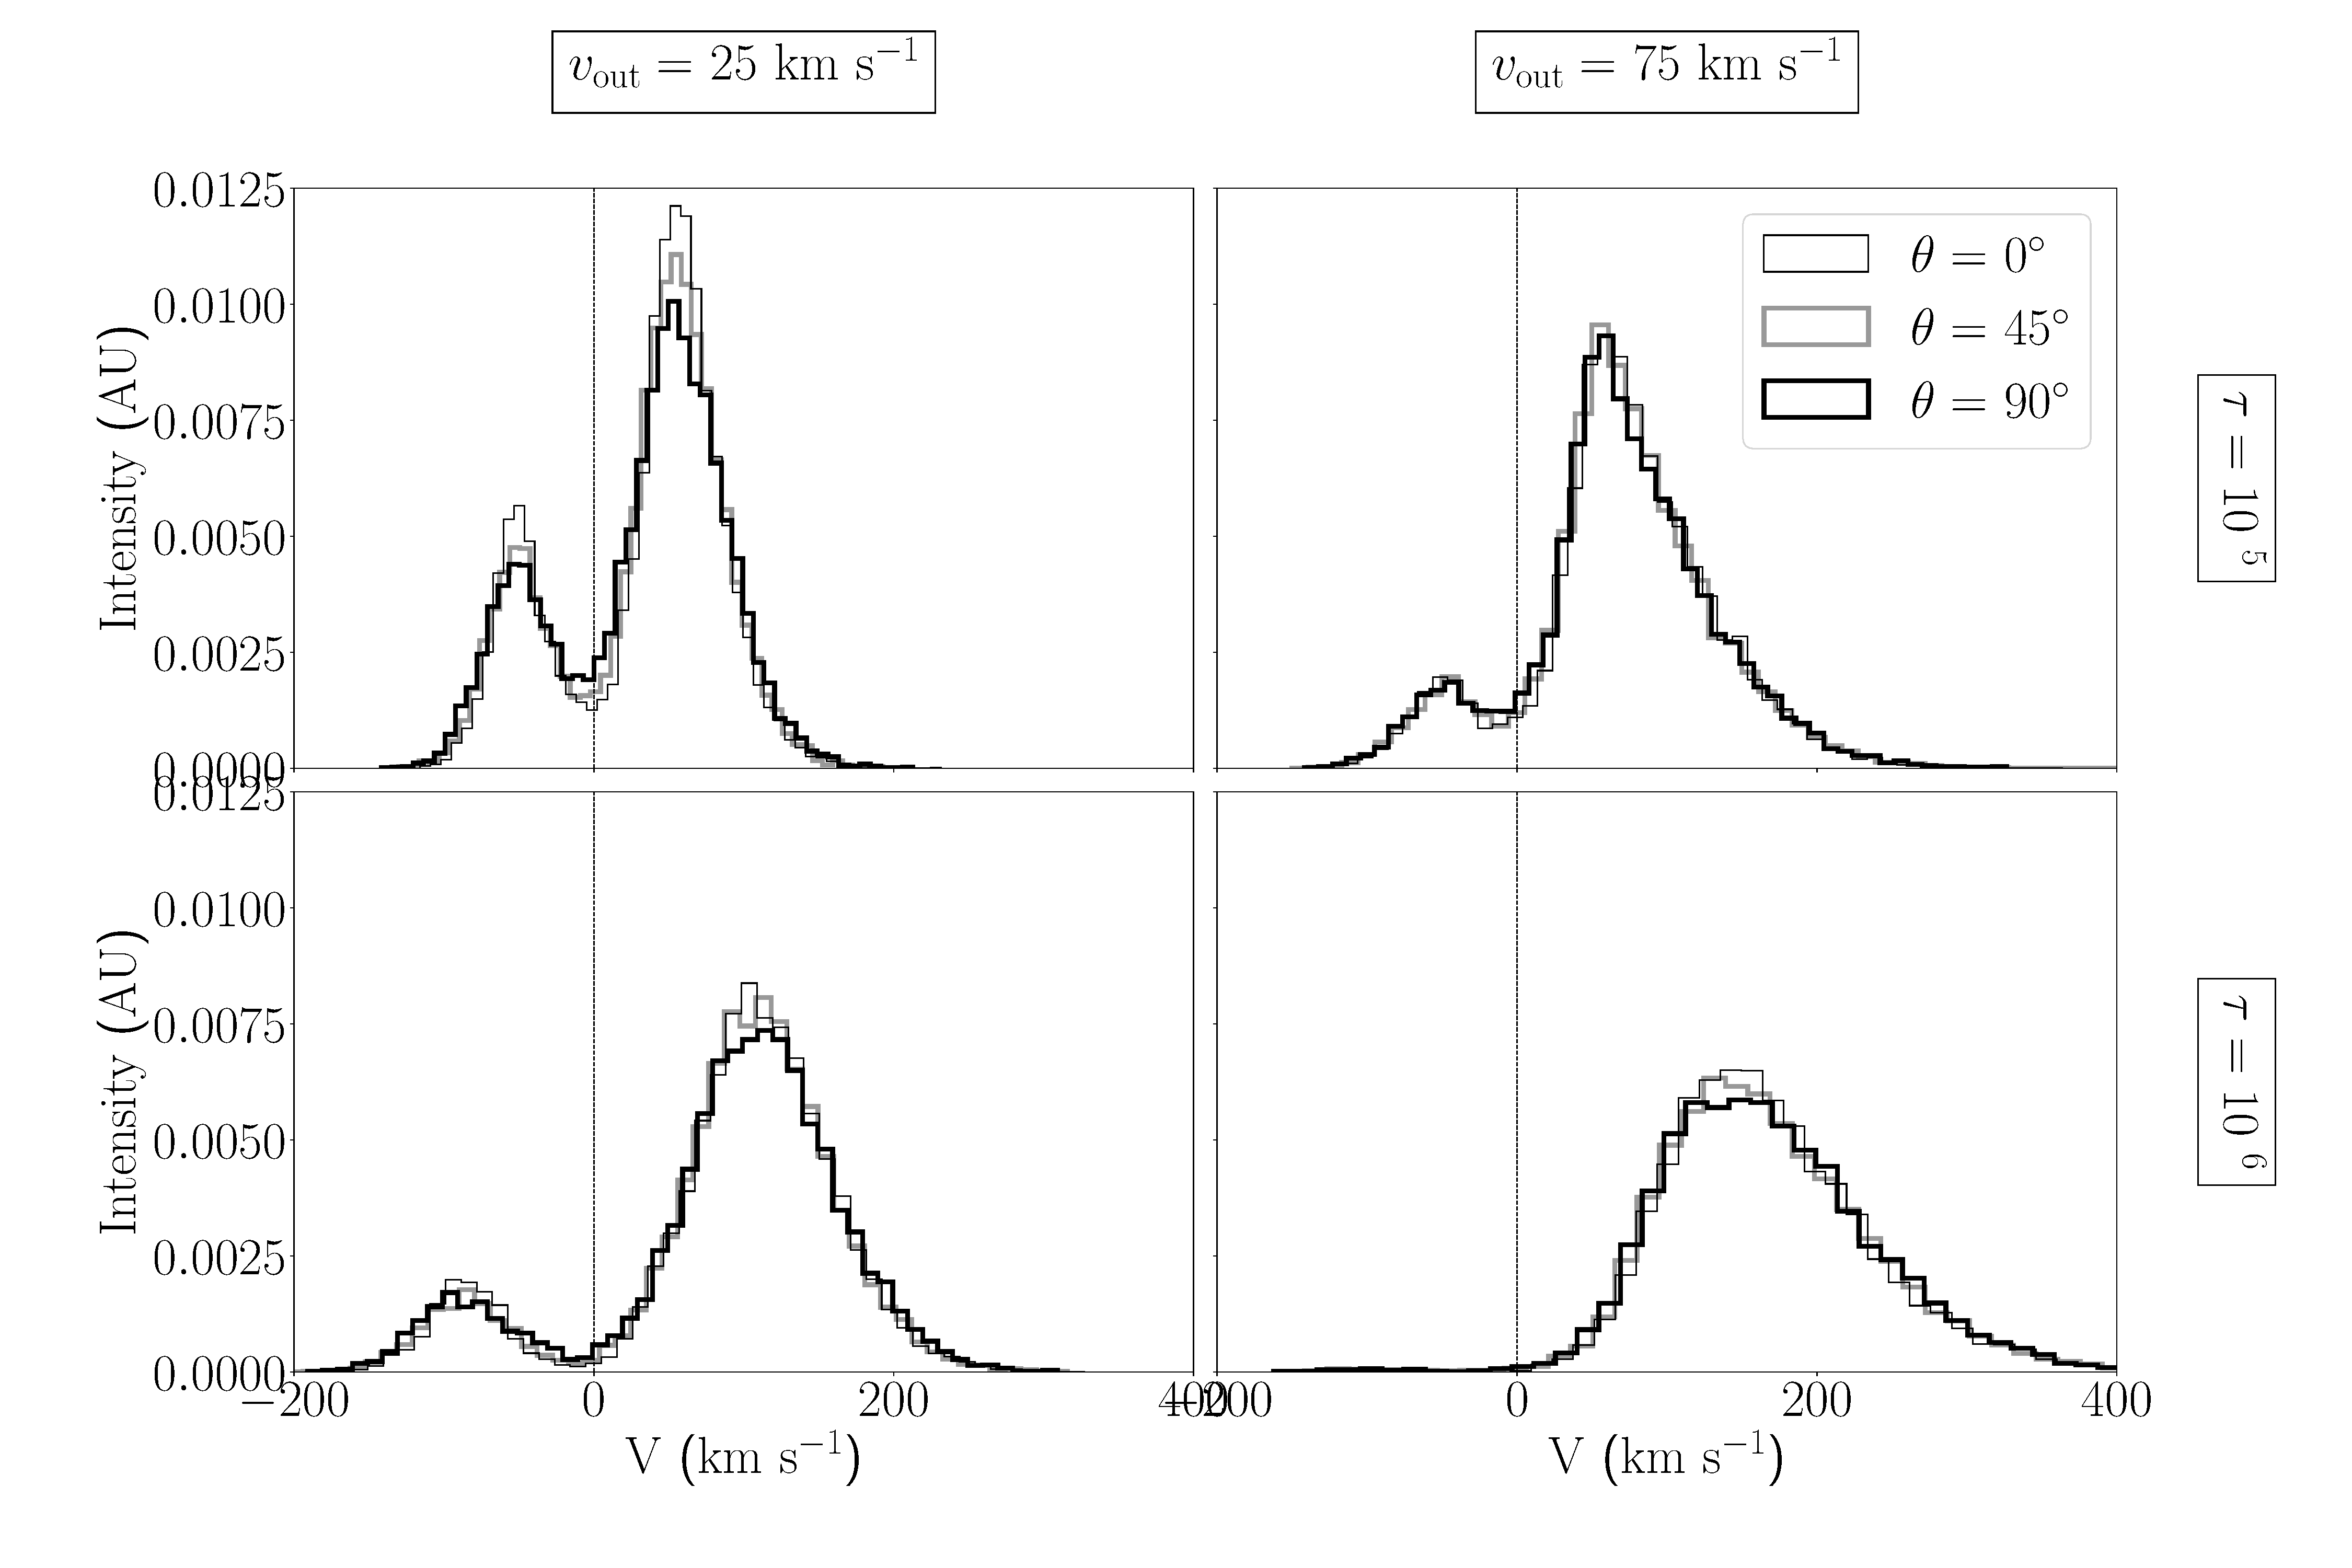
\includegraphics[width=0.90\textwidth]{./figures/appendix/varying_outflow_small}
	\end{center}
	\caption{\textbf{Spectra with fixed rotation velocity:} We fix $\vrot=50$\kms.
		\label{fig:varying_outflow_small}}
\end{figure*}

% Esta figura deberia tener 3 x 3 vinetas. vout=50.
% cada panel tiene una curva para theta=0, 45, 90.
% |tau=1E5, vrot=0, | tau=1E5, vrot=50, | tau=1E5, vrot=100,
% |tau=1E6, vrot=0, | tau=1E6, vrot=50, | tau=1E6, vrot=100,
% |tau=1E7, vrot=0, | tau=1E7, vrot=50, | tau=1E7, vrot=100,
\begin{figure*}
	\begin{center}
		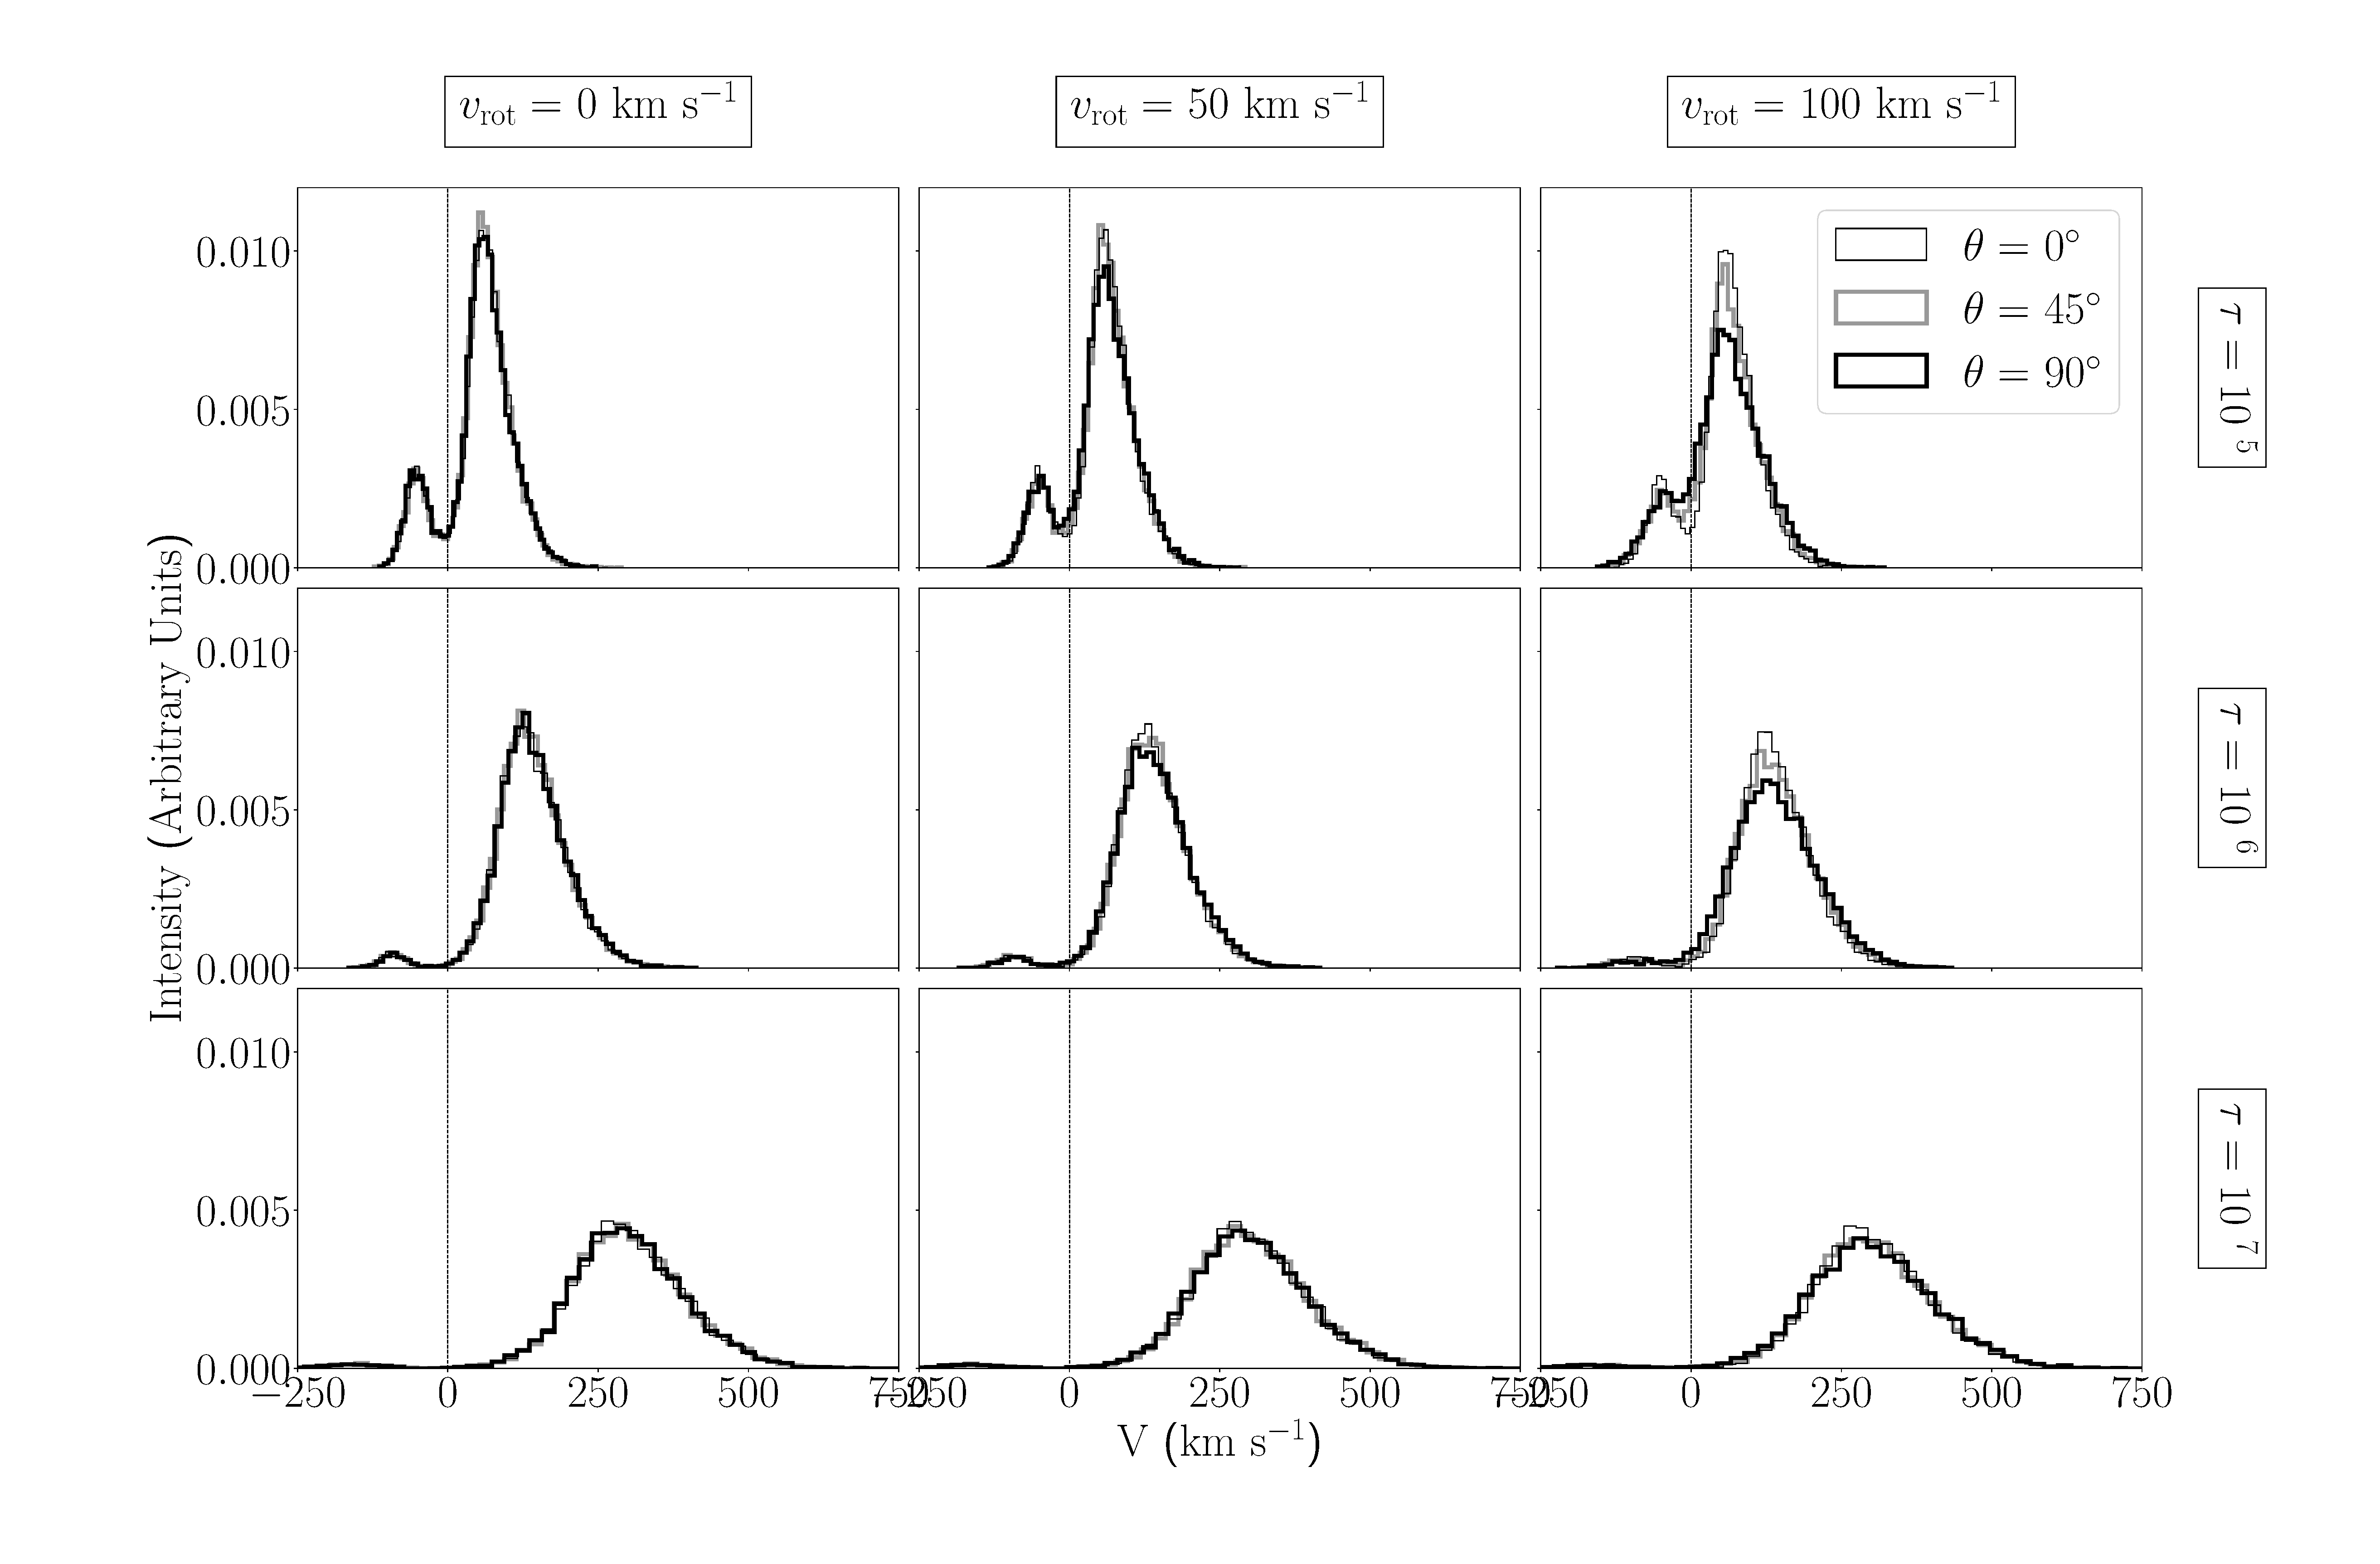
\includegraphics[width=0.90\textwidth]{./figures/appendix/varying_rotation}
	\end{center}
	\caption{\textbf{Spectra with fixed outflows velocity:} We fix $\vout=50$\kms.
		\label{fig:varying_rotation}}
\end{figure*}

% Esta figura deberia tener 3 x 3 vinetas. vrot=50.
% cada panel tiene una curva para theta=0, 45, 90.
% |tau=1E5, vout=25, | tau=1E5, vout=50, | tau=1E5, vout=75,
% |tau=1E6, vout=25, | tau=1E6, vout=50, | tau=1E6, vout=75,
% |tau=1E7, vout=25, | tau=1E7, vout=50, | tau=1E7, vout=75,
\begin{figure*}
	\begin{center}
		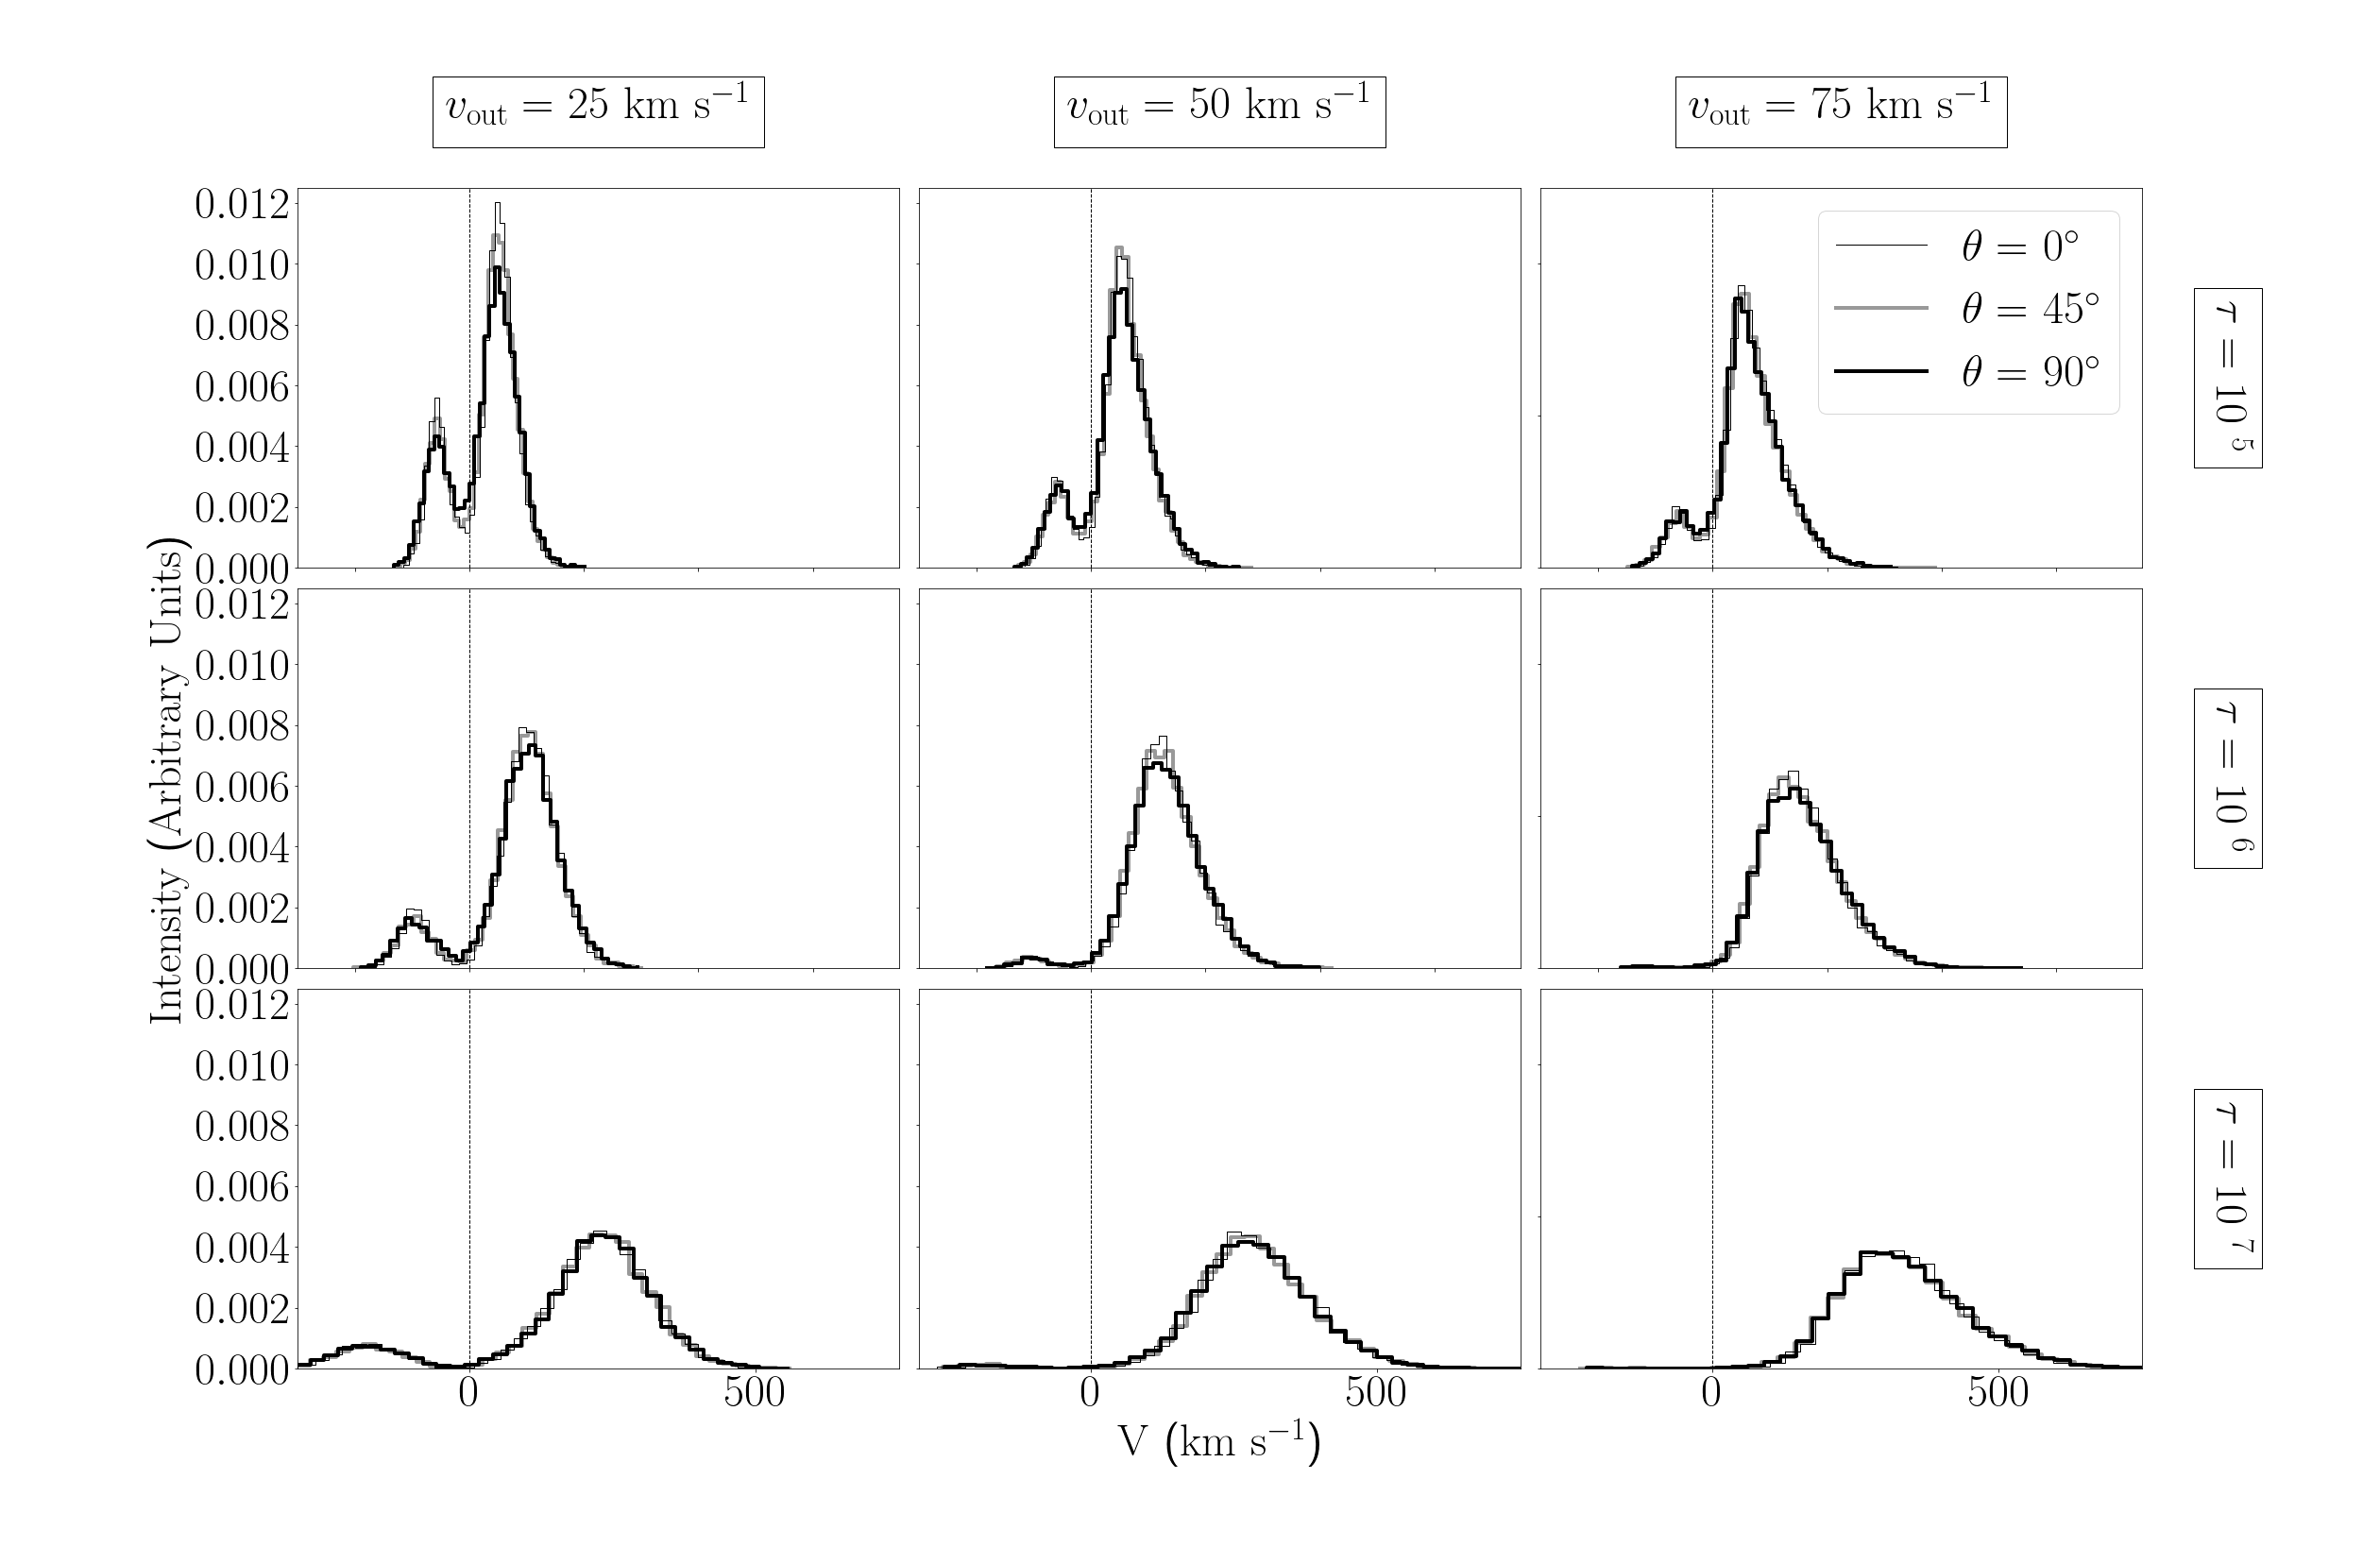
\includegraphics[width=0.90\textwidth]{./figures/appendix/varying_outflow}
	\end{center}
	\caption{\textbf{Spectra with fixed rotation velocity:} We fix $\vrot=50$\kms.
		\label{fig:varying_outflow}}
\end{figure*}



\end{document}


\cite{DjorgovskiThompson}, \cite{Rhoads00},
\cite{Gawiser2007}, \cite{Koehler2007}, \cite{Ouchi08},
\cite{Yamada2012}, \cite{Schenker2012}, \cite{Kulas12},
\cite{Yamada2012}, \cite{Chonis2013}, \cite{Finkelstein2013},
\cite{Ostlin14}, \cite{Hayes2014}, \cite{Faisst2014},
\cite{Fumagalli2015}.


\section{A new LAE model}

(\cite{Adams72}, \cite{Harrington73}, \cit
e{Neufeld90}, \cite{Dijkstra06}, \cite{Verhamme06}, \cite{Forero12},
\cite{Martin2015}, \cite{Garavito14}, \cite{Neufeld91},
\cite{Laursen09}, \cite{Barnes11}, \cite{Verhamme12},
\cite{Yajima12}).\\


\subsection{Galaxy's Viewing Angle}

We illustrate this in
Fig. \ref{fig:model}. \\

\begin{figure}[h!]
  \begin{center}
    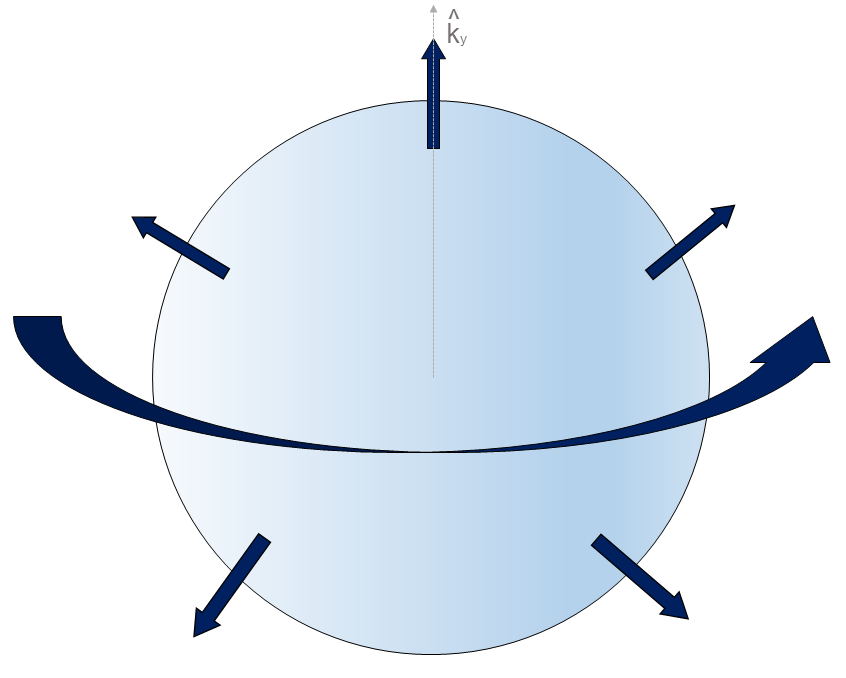
\includegraphics[width=0.48\textwidth]{./figures/model}
  \end{center}
	\caption{\textbf{Model:} Spherical LAE with tangential and radial velocities due to rotation and outflows, respectively. The galaxy cut is in the $y-z$ plane perspective. The observer is located at an specific viewing angle of the sphere. Only photons with a direction that enters in this range of vision are taken into account to build the observed spectrum.
		\label{fig:model}}
\end{figure}


\section{Results}

\subsection{Resulting simulated spectra}
In order to define the ranges of tauh, vrot and vout, it is necessary
to refer to observational constraints. The common values for typical
LAEs that were set as parameters are in Tab. \ref{tab:values}. We run
CLARA's modified version for all the permutations of these 3
parameters. \\

The behavior of the resulting sets of spectra can be summarized by
Fig. \ref{fig:summary}. We concluded from the simulations a clear
creation of two asymmetric peaks around $V=0$ \kms with the tallest
peak always redshifted. We detected a strong dependence on the outflow
velocity that induces the peak asymmetry. We also detected that the
rotation velocity broadens the line horizontally. Both these effects
have been previously reported separately in the literature, so these
results can valid their superposition to some extend. \\

\begin{figure}[h!]
	\begin{center}
		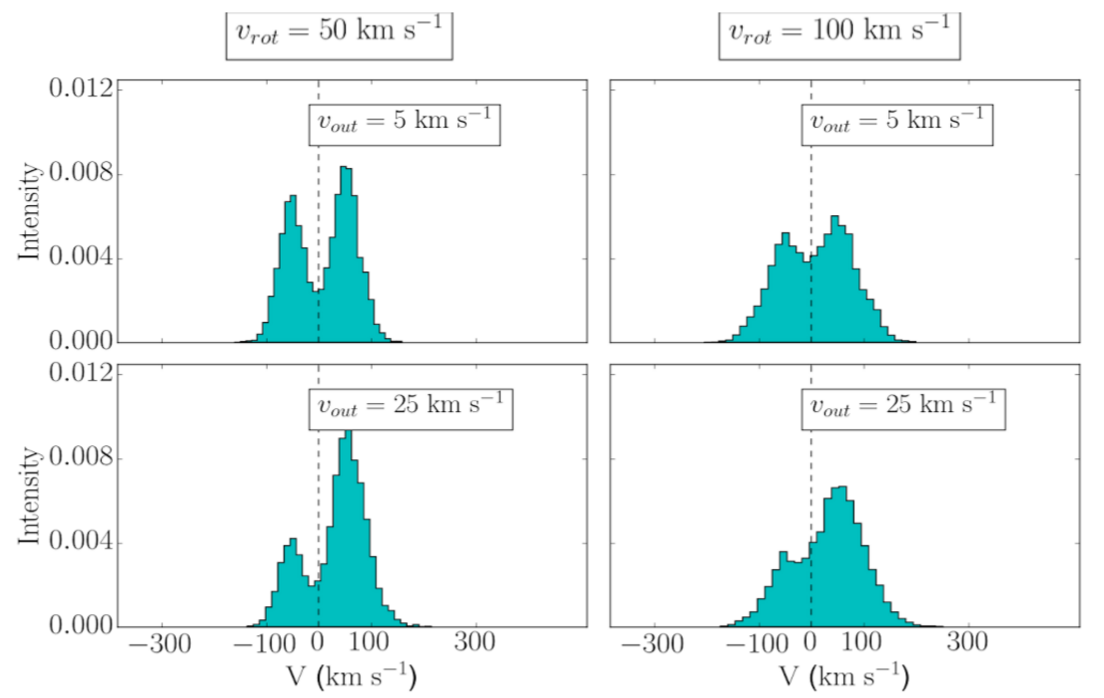
\includegraphics[width=0.48\textwidth]{./figures/summary}
	\end{center}
	\caption{\textbf{4 different \lya profiles:} With tauh$=10^5$ and $\theta \simeq 90^\circ$. The rotational velocity vrot increases to the right and the outflows velocity vout increases downwards. The intensity is in arbitrary units.
		\label{fig:summary}}
\end{figure}

\subsection{Influence of the viewing angle $\theta$}
We take now into account the viewing angle of the galaxy to build the observed spectra. For all of the physical parameters' combinations, the effect of $\theta$ in the \lya line is always the same.\\

\begin{figure}[h!]
	\begin{center}
		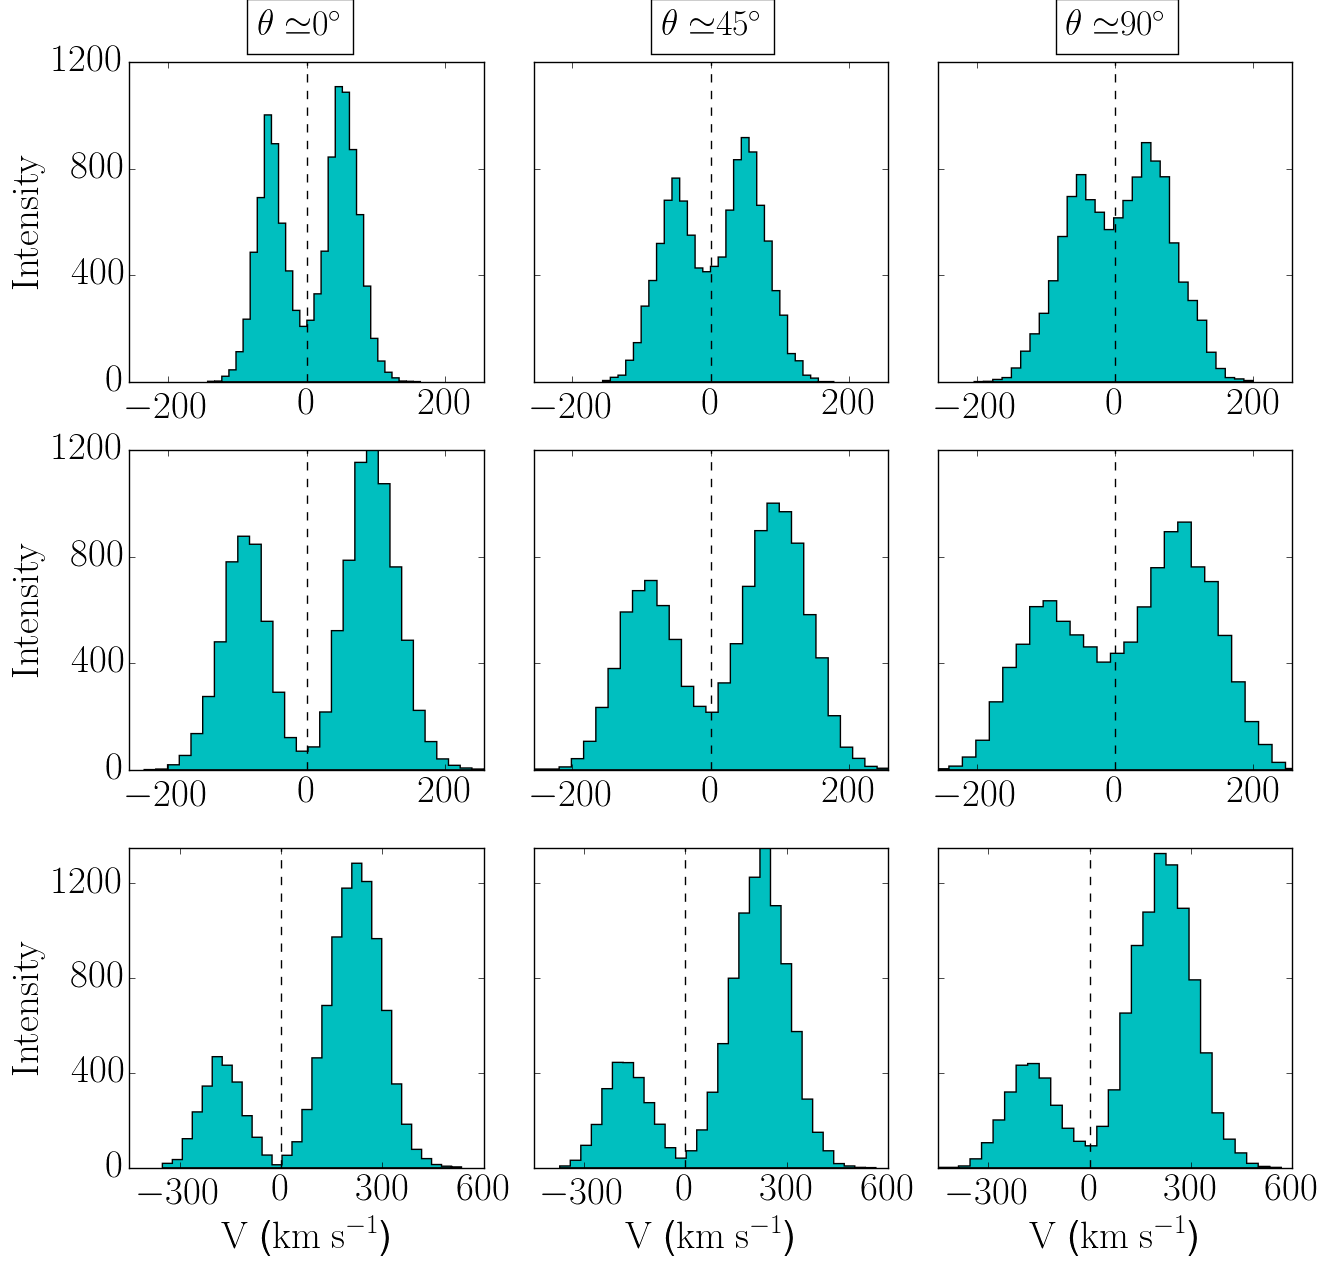
\includegraphics[width=0.5\textwidth]{./figures/angles}
	\end{center}
	\caption{\textbf{\lya profile for different $\theta$.} For tauh$=10^5$, vrot$=50$ \kms and vout$=20$ \kms. For tauh$=10^6$, vrot$=100$ \kms and vout$=5$ \kms. For tauh$=10^7$, vrot$=100$ \kms and vout$=15$ \kms. The intensity is in arbitrary units.
		\label{fig:angles}}
\end{figure}

From Fig. \ref{fig:angles} it is clear that the intensity of the valley between the two peaks increases along with $\theta$. This causes an intensity decrease in the rest of the frequencies, thus a broadening of the line. The asymmetry also changes with the viewing angle.\\


\subsection{Morphology of \lya line}

To summarize, the influence of the 4 parameters on the \lya morphology is the following:

\begin{itemize}
	\item tauh induces a redshift. Increasing the optical depth separates the line of the zero velocity line. \\
	\item vout decreases the right peak's intensity. Higher vout makes the left peak smaller until it merges with the right one. \\
	\item vrot broadens the line and decreases the maximum intensity. Higher vrot implies a flatter spectrum. This effect has not been deeply studied in literature. Only Garavito et al. \cite{Garavito14} has simulated its effect. Our results are consistent with their conclusions.
	\item $\theta$ increases the central valley of the line. Higher $\theta$ makes more emission at \lya natural frequency. \\
\end{itemize}

\subsection{Doppler shift by rotation}

The rotation effect induces a Doppler shift in frequency and displaces the only-outflows spectra. As seen in Fig. \ref{fig:rotation_doppler_outflow} rotation takes the resulting spectrum with vrot$=0$ and displaces it from its central location. Then it weights the lines and they all merge into the resulting red \lya line.\\

\begin{figure}[h!]
	\begin{center}
		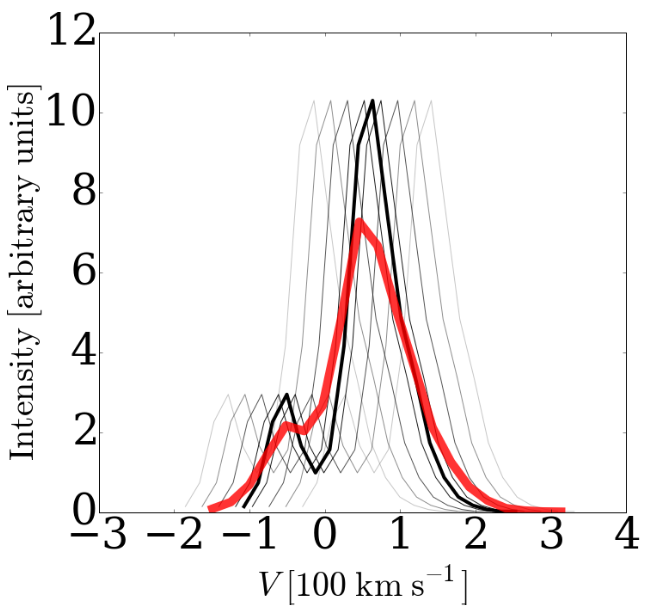
\includegraphics[width=0.3\textwidth]{./figures/rotation_doppler_outflow}
	\end{center}
	\caption{\textbf{Rotations induces a Doppler shift of the only-outflows spectra:} Each of the black lines is then weighted to obtain the red line.
		\label{fig:rotation_doppler_outflow}}
\end{figure}

PONER GRAFICA REAL...\\

\section{Observational Implications}

Among the observational implications that this paper has over observations we select three principal ones. First, the rotational effects of the galaxy should be clearly detected and characterized by MUSE's high resolution data. The Doppler redshift is already visible in other observations, such as the one seen in Fig. 7 of Prescott et al. \cite{Prescott14}.\\

Second, the central ($V=0$) emission of the spectra seen in the results is a consequence of the viewing angle of the galaxy and can be controlled by it. This means that the reason is not necessary that radiation is escaping without scattering, as several authors have suggested (CITAS...).\\

Finally, all the spectra produced from this new LAE model is roughly consistent with observations. The consideration of adding the new rotation parameter to the standard only-outflows model found in literature is reasonable and very powerful. vrot and its consequent viewing angle $\theta$ can modify the morphology of the \lya line in new different ways by keeping the model simplified.\\

\section{Conclusions}

In this paper, the objective was to analyze and measure the influence
of galaxy rotation and outflows on the \lya line. The motivation for
this is to be able to obtain physical information of a LAE by just
looking at its \lya profile. In order to accomplish this objective, we
propose a new model of a LAE consisting of a sphere of Hydrogen atoms
that expands radially and rotates as a solid body. A modified version
of the program CLARA \cite{CLARA} is used to set the conditions and
emulate the radiative transfer process inside the galaxy. \\ 

The conclusions obtained from this work are:

\begin{itemize}
	\item The outgoing spectra depend on the angle an external observer is viewing the galaxy from. The closer it is to the equator of the galaxy, the higher the central valley of the frequency distribution.

	\item The effects of vrot, vout and tauh are consistent with the different authors that have used them. vrot broadens the \lya line. vout increases the peaks asymmetry and tauh induces a redshift around the zero velocity.

	\item Rotations induces a Doppler shift in frequency of the only-outflows spectra.

	\item The final spectra obtained are roughly consistent with LAEs observations. \\

\end{itemize}

\subsection{Future work}

For future work regarding the model, we would like to implement a differential rotation for the LAE instead of solid body. Regarding result analysis, we would like to compare against observations in two ways. Firstly by using the kinematic observation obtained from newly observed LAEs. We could do a consistency check between their real spectra and the simulated one that our model would produce with the respective parameters. Secondly we would like to take a specific observed spectrum and fit it using MCMC in order to predict ranges for its parameters. \\

\subsection{Reproducibility}

All of this work is available online and free to use to anyone. The data, source code and instructions to replicate this paper's results are in the GitHub repository:  \texttt{github.com/astroandes/CLARA\_RotationOutflows}. \\


\section*{Acknowledgments}
The authors would like to acknowledge the high performance computational cluster (HPC) hosted by Universidad de los Andes, where we ran the simulations for CLARA. \\

We would also like to acknowledge the participants of the meeting \textit{Escape of Lyman radiation from galactic labyrinths} at Crete, Greece, for their valuable comments on this work, specially to Max Gronke and Christian Herenz. \\


%------------------------REFERENCES----------------------------
